% Useful references:
% - https://www.overleaf.com/learn/latex/How_to_Write_a_Thesis_in_LaTeX_(Part_1)%3A_Basic_Structure
\documentclass[
	a4paper, 		% a4 page format
	12pt,			% font size: note 12 pt -> \footnotesize is set at 10pt
	openright,		% (openany|openright) starts a chapter on the next available page or always on a right page
	twoside,		% front and back print
	titlepage,		% (titlepage|notitlepage)
]{book}				% see https://tex.stackexchange.com/questions/36988/regarding-the-book-report-and-article-document-classes-what-are-the-mai
%
\usepackage{thesis-style}
%
\addbibresource{bibliography.bib}	% Imports bibliography file
%
\begin{document}
	% --------------------------------------------------------------------
	% Frontmatter makes the pages numbered in lowecase roman and make 
	% chapters not numbered, although each chapter's title appears in the
	% table of contents.
	% --------------------------------------------------------------------
	\frontmatter
	% ! TeX root = thesis.tex
\begin{titlepage}
    \begin{center}
        {\Large
            \textbf{
                \textsc{Alma Mater Studiorum $\cdot$ Universit\'a di Bologna}
            }
        }
        {\large
            \textbf{
                \textsc{Campus di Cesena}
            }
        }
        \rule[0.1cm]{15.8cm}{0.1mm}
        \rule[0.5cm]{15.8cm}{0.6mm}
        {\Large
                Dipartimento di informatica $-$ Scienza e Ingegneria \\
        }
        \vspace*{4mm}
        {\Large 
            Corso di Laurea in Ingegneria e Scienze Informatiche
        }
        \vspace*{15mm}
        \begin{center}
            {\LARGE
                \textbf{
                    TITOLO TESI
                }
            } \\
            \vspace*{15mm}
            {\Large
                Elaborato in 
            } \\
            \vspace*{3mm}
            {\Large
                \textsc{Programmazione ad Oggetti}
            }
        \end{center}
        \vspace*{40mm}
    \end{center}
\end{titlepage}
	% ! TeX root = thesis.tex
\begin{abstract}
    Lo scopo di questa tesi...
\end{abstract}
	%% ! TeX root = ../../thesis.tex
\begin{dedication}
    Dedica...
\end{dedication}

	\tableofcontents
	\listoffigures
	\lstlistoflistings
	% --------------------------------------------------------------------
	% Mainmatter command changes the behavior back to the expected version, 
	% and resets the page number.
	% --------------------------------------------------------------------
	\mainmatter
	% ! TeX root = ../../thesis.tex
\chapter{Contesto e motivazioni}
\label{chapter:context-and-motivations}

\todo{introduzione}

\section{Il problema del plagio nel software}

\todo{definisce il problema, eventuali sottocapitoli che spiegano come è diviso}

\section{Sistemi antiplagio automatici}

\todo{spiegare cosa esiste e perché serve che sia automatico}

\section{Stato dell'arte}
% preso spunto da "Current trends in source code analysis, plagiarism detection and issues of analysis big datasets" -- si deve citare??
Il codice sorgente non è nient'altro che un file di testo scritto da sviluppatori, che deve essere compilato o interpretato e che, pertanto, si basa su regole sintattiche e grammaticali proprie del linguaggio di programmazione con cui è scritto che permettono a entrambi gli attori, il programmatore e il calcolatore, di "capirlo" ed elaborarlo.

Per questo motivo, se processare la struttura di un sorgente non presenta grandi difficoltà, processare il significato, ovvero l'idea e la logica sottesa al codice, costituisce una sfida più grande, se non altro perché entra in gioco la competenza dello sviluppatore e la sua esperienza nella scrittura di codice "pulito".

Poiché il problema è complesso, gli attuali metodi di analisi non aspirano a risolvere il problema \textit{in toto}, ma analizzano il codice sorgente utilizzando particolare "punto di vista": alcuni analizzano il codice dal punto di vista del programmatore, cercando di comprenderne il significato, altri la loro struttura.

% Possiamo classificare le tecniche di analisi in tre approcci: 

% Il primo si basa sull'analisi del codice come mero testo: si presume che siano rispettate le convenzioni e il codice contenga sufficienti informazioni che ne descrivano il significato e cercano di estrarre solo queste significative informazioni aggiuntive.

% Il livello successivo è simile al precedente con la differenza che non esplora il significato del testo dal punto di vista del programmatore, bensì dal punto di vista del calcolatore, che "vede" il codice come una sequenza di comandi, ciascuno con il proprio significato nel contesto della grammatica del linguaggio.

% L'ultimo e terzo livello riguarda l'analisi del modello del codice sorgente.

In generale, come già accennato nel \todo{ref?}, la maggior parte dei sistemi automatici d'identificazione di plagi lavorano in due fasi consecutive: prima il codice sorgente viene analizzato e viene generata una rappresentenzazione intermedia, poi si effettua il confronto dei sorgenti sulle rappresentazioni intermedie.

Le tecniche di analisi possono essere classificate in tre cataegorie: \textbf{\textit{structure-based}}, \textbf{\textit{attribute-based}}, \textbf{\textit{hybrid detection}}. \todo{citazione?}

\subsection{Analisi \textit{structure-based}}

\subsubsection{Analisi lessicale}
Tra tutte, la tecnica più usata consiste nell'analisi lessicale (\textbf{\textit{lexical analysis}} o \textbf{\textit{tokenization}} in inglese) del codice sorgente, che consiste nel convertire la sequenza di caratteri di cui è composto il programma in una sequenza di \textit{token}.
%
Un \textit{token} è una sequenza di caratteri che costituisce un'unità fondamentale nella grammatica del linguaggio ed è strutturato come una coppia \textit{nome} - \textit{valore}.
%
Alcuni possibili esempi sono riportati in \Cref{table:token-examples}.

\begin{itemize}
    \item \textit{identifier}: una stringa di lettere e numeri che iniziano con una lettera (usato per rappresentare i nomi scelti dai programmatori);
    \item \textit{keyword}: stringa per rappresentare i nomi dedicati nella sintassi del linguaggio;
    \item \textit{separator}: caratteri delimitatori e di punteggiatura;
    \item \textit{comment}: blocco di commenti.
\end{itemize}

\begin{table}[h]
    \centering
    \begin{tabular}{|c|c|} 
        \hline
        \textbf{Nome} & \textbf{Esempi di valori} \\ [0.5ex] 
        \hline\hline
        \textit{identifier} & \texttt{x}, \texttt{name}, \texttt{color} \\ 
        \hline
        \textit{keyword} & \texttt{if}, \texttt{for}, \texttt{return} \\
        \hline
        \textit{separator} & \texttt{\{}, \texttt{\}}, \texttt{(}, \texttt{;} \\
        \hline
        \textit{comment} & \texttt{/* This is a sample comment */} \\
        \hline
    \end{tabular}
    \caption{Esempi di possibili coppie nome-valore di \textit{token} comuni.}
    \label{table:token-examples}
\end{table}

L'analisi lessicale rappresenta il primo stadio della struttura di un compilatore ed è eseguita da programmi denominati \textbf{\textit{lexer}}. 
%
Questi sono generati in maniera dichiarativa a partire da generatori di \textit{lexer} (\textbf{\textit{lexer generator}}) che, presi in input più automa a stati finiti, espressi per mezzo di espressioni regolari che definiscono in maniera formale la grammatica del linguaggio, generano il codice che implementa l'algoritmo di analisi lessicale. 
% https://www.antlr.org ??

Attraverso questo approccio, quindi, ogni programma viene trasformato in una sequenza di \textit{token}, uno per ciascun elemento di base del linguaggio che si vuole valorizzare: i blocchi di commenti o documentazione, gli \texttt{import} e altre sezioni di codice non rilevanti ai fini della comparazione possono essere esclusi, cioè non viene generato alcun \textit{token} per questi elementi.
%
Questo li rende insensibili contro le modifiche ma \dots

\todo{esempio di tokenizzazione applicata a un sorgente}

In seguito, la sequenza di \textit{token} generata viene confrontata con algoritmi di \textit{string matching}.

\subsubsection{Analisi basata su un modello}
Invece di utilizzare la mera sequenza di \textit{token} generata dal generatore di \textit{lexer} possono essere generate delle strutture e dei modelli più complessi.

Il più diffuso è l'\textbf{albero sintattico} (o \textit{abstract syntax tree} in inglese, abbreviato AST).

\dots

Program Dependency Graph

\subsection{Analisi \textit{attribute-based}}
Nonostante l'efficienza delle tecniche di analisi strutturale descritte precedentemente, il loro punto debole si riscontra nelle prestazioni. 
%
Per far fronte a questo problema sono state storicamente introdotte nuove tecniche, dette \textit{attribute-based}, in quanto determinano il grado di similarità tra due sorgenti sulla base delle loro \dots

\subsection{\textit{Hybrid detection}}

\subsection{Quale tecnica scegliere?}
In conclusione, scegliere quali di questi approcci scegliere è complesso, perché difficili da confrontare tra loro: la maggior parte di queste tecniche viene valutata utilizzando il proprio \textit{set} di dati, che raramente sono resi pubblicamente accessibili \cite{karnalim-budi-toba-joy-2019}.

In conclusione, bisogna rendersi conto che, a prescindere dal grado di sofisticatezza della tecnica che si utilizza, è sempre possibile che si verifichi un plagio non rilevabile.
%
Da bilanciare le risorse investite nell'individuazione del plagio e i rendimenti decrescenti di trovare i pochi, se non nessuno, casi difficili da rilevare \cite{joy-99}.



	% ! TeX root = ../../thesis.tex
\chapter{Analisi e Progettazione}
\label{chapter:analysis}
In questo secondo capitolo viene presentata l'analisi dei requisiti e il \textit{design} del sistema.
%
Nei primi due paragrafi vengono elencati i requisiti ed è descritto il dominio applicativo.
%
Il terzo paragrafo è dedicato alla progettazione dello strumento: si parte da una visione architetturale e a seguire si dettagliano le parti di \textit{design} più rilevanti al fine di chiarificare la logica con cui è stato implementato il sistema.

\section{Requisiti}
Come già anticipato, lo scopo della tesi è realizzare un sistema antiplagio automatico in grado d'individuare eventuali porzioni di codice copiato nei progetti \textit{software} del corso di Programmazione ad Oggetti dell'Università di Bologna.

Di seguito vengono descritti, per punti, i requisiti del sistema, suddivisi tra requisiti \textit{funzionali} e \textit{non funzionali}.

\subsection*{Requisiti funzionali}
\begin{itemize}
    \item Il sistema riceve in \textit{input} un insieme di progetti di cui si vuole verificare l'autenticità, detto \textbf{\textit{Submission}}, e un insieme di progetti con cui confrontarli, detto \textbf{\textit{Corpus}};
    
    \item Il confronto viene effettuato tra progetti sviluppati nello stesso linguaggio di programmazione: Java.
    
    \item I progetti sono mantenuti in \textit{repository} pubbliche su \textit{GitHub} e \textit{Bitbucket}\footnote{
        \href{https://github.com}{\textit{GitHub}} e \href{https://bitbucket.org}{\textit{Bitbucket}} sono due tra i più conosciuti servizi di \textit{hosting} per progetti \textit{software} che utilizzano sistemi di controllo di versione decentralizzati, come \href{https://git-scm.com}{Git}.
    }. Si assume che i progetti passati siano tempo-invarianti: dal momento in cui vengono corretti, le rispettive \textit{repository} sono archiviate e mai più modificate;

    \item Il sistema deve fornire in \textit{output} le sezioni di codice che, con un determinato livello di accuratezza, ha stabilito essere simili.
\end{itemize}

\subsection*{Requisiti non funzionali}
\begin{itemize}
    \item L'algoritmo per determinare la similarità, così come le metriche utilizzate, devono essere interscambiabili, facilmente estendibili e configurabili da parte dell'utente;
    \item Le informazioni estrapolate dai sorgenti sono salavate in modo tale da essere riutilizzate nelle analisi successive di altri progetti;
    \item \`E necessario che il sistema impieghi un tempo "ragionevole" per effettuare la computazione.
\end{itemize}

\section{Analisi e modello del dominio}
Il sistema deve essere in grado, a partire da un insieme di \texttt{Repository}, corrispondenti a progetti coerenti per linguaggio di programmazione, di estrarne una rappresentazione confrontabile (\texttt{SourceRepresentation}) medianti opportuni algoritmi di analisi (\texttt{Analyzer}).
%
Ciascuna coppia di rappresentazioni intermedie deve essere successivamente filtrata per mezzo di un apposito \texttt{Filter} e confrontata tramite algoritmi di rilevamento di somiglianze (\texttt{PlagiarismDetector}) al fine di poter determinare eventuali parti di codice duplicato e/o somiglianze, generando infine dei \texttt{report}.

Gli elementi costitutivi il problema sono sintetizzati in \Cref{img:02-domain}.

La principale difficoltà sarà individuare tecniche di analisi e di rilevamento delle somiglianze che siano robuste, ovvero permettano d'identificare casi di copiature anche se lo sviluppatore ha effettuato modifiche per offuscarle.
%
Particolare attenzione dovrà essere posta sulla progettazione dei componenti per l'analisi e per il confronto, in quanto, data la natura del sistema, possono dover cambiare frequentemente ed essere fortemente configurabili.
%
Inoltre, il requisito non funzionale sulle \textit{performance} richiederà un'analisi dei tempi di esecuzione non appena il sistema sarà completato.

\begin{figure}[h!]
    \centering
    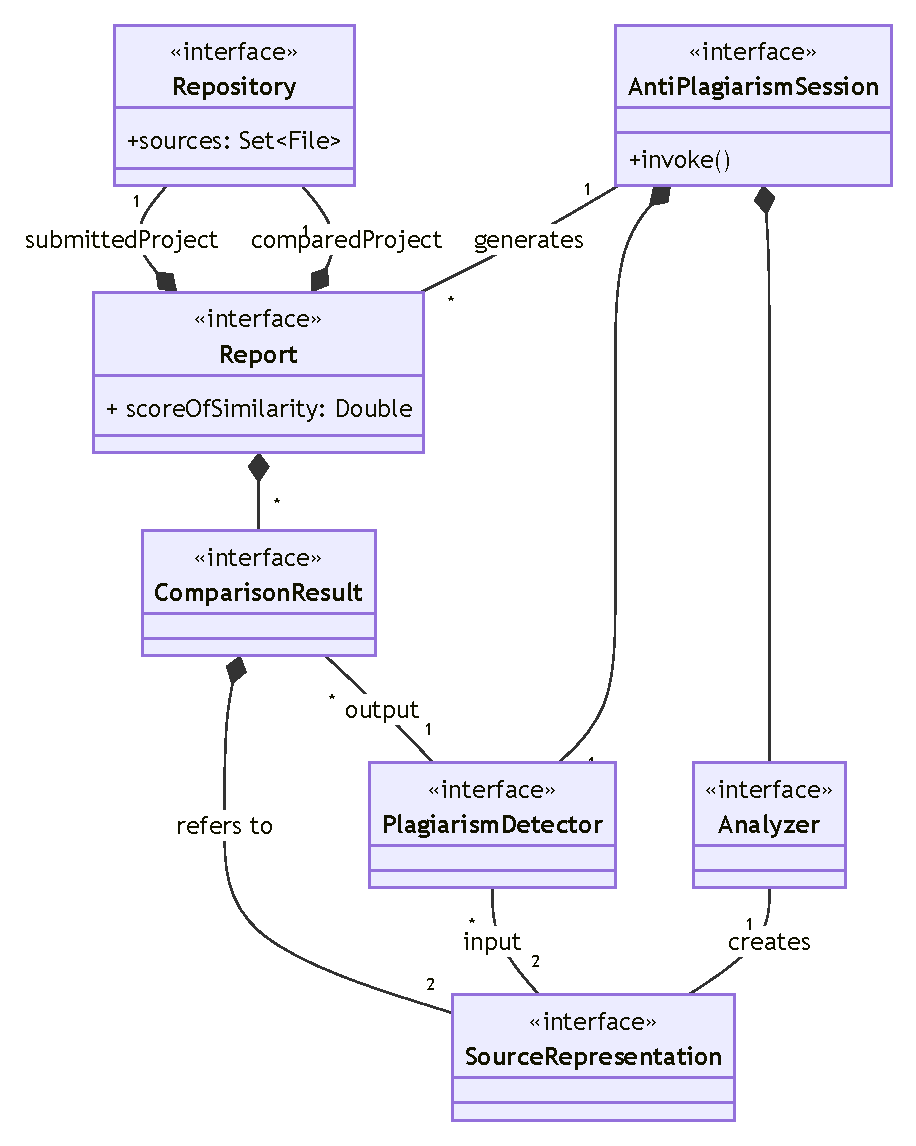
\includegraphics[width=0.9\textwidth]{resources/img/02-domain.pdf}
    \caption{Schema UML delle classi dell'analisi del problema, con rappresentate le entità principali ed i rapporti fra loro.}
    \label{img:02-domain}
\end{figure}

\section{\textit{Design}}

\subsection{Architettura}
%
% --- inizio da rivedere! ---
% manca la trattazione degli input e su come viene configurato, nonché la gestione del salvataggio.
%
L'architettura del sistema è così organizzata: \textbf{\texttt{AntiPlagiarismSession}} è l'interfaccia responsabile della logica dell'applicazione e rappresenta una specifica sessione, dove per sessione si intende l'entità che, una volta opportunamente configurata, esegue la logica dell'applicazione.

Gli \texttt{Output} rappresentano le risorse su cui andare a rappresentare i risultati ottenuti, mentre il \texttt{RepositoryProvider} rappresenta la strategia con cui recuperare i progetti su cui effettuare l'analisi.

Il confronto e l'analisi dei sorgenti vengono effettuati, rispettivamente, dal \texttt{PlagiarismDetector} e dall'\texttt{Analyzer}, che incapsula la specifica strategia utilizzata e demanda a \texttt{KnoledgeBaseRepository} il salvataggio e il recupero delle rappresentazioni dei sorgenti già precedentemente analizzati e, perciò, salvati.

Questa architettura permetterebbe facilmente l'aggiunta di un nuovo \texttt{Output} e di poter cambiare sia la strategia per recuperare i progetti, sia la logica con cui questi vengono processati.

In \Cref{img:02-architecture} è esemplificato il diagramma UML architetturale.

\begin{figure}[h!]
    \centering
    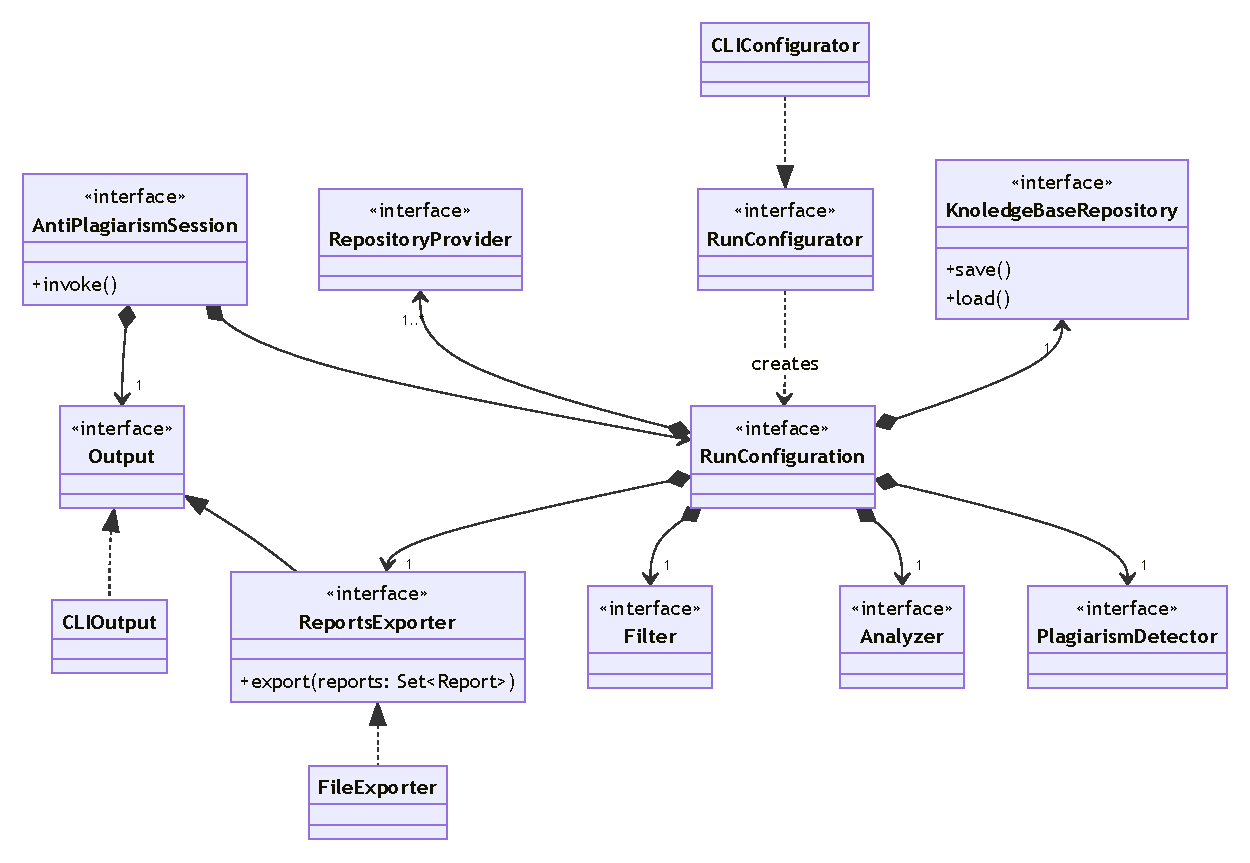
\includegraphics[width=\textwidth]{resources/img/02-achitecture.pdf}
    \caption{Schema UML architetturale del sistema.}
    \label{img:02-architecture}
\end{figure}
%
% --- fine da rivedere ---
%

\subsection{\textit{Design} dettagliato}

\subsubsection*{\textit{Provider} dei progetti}
Per quanto concerne i \textit{provider} di \textit{repository}, ovvero i componenti che devono recuperare i sorgenti dei progetti da \textit{repository} pubbliche da \textit{GitHub} e/o da \textit{Bitbucket}, si è scelto un \textit{design} che permettesse il massimo riuso degli elementi comuni, aderendo a uno schema interfaccia $-$ classe astratta $-$ classe concreta (\Cref{img:02-provider}).

\begin{figure}[h!]
    \centering
    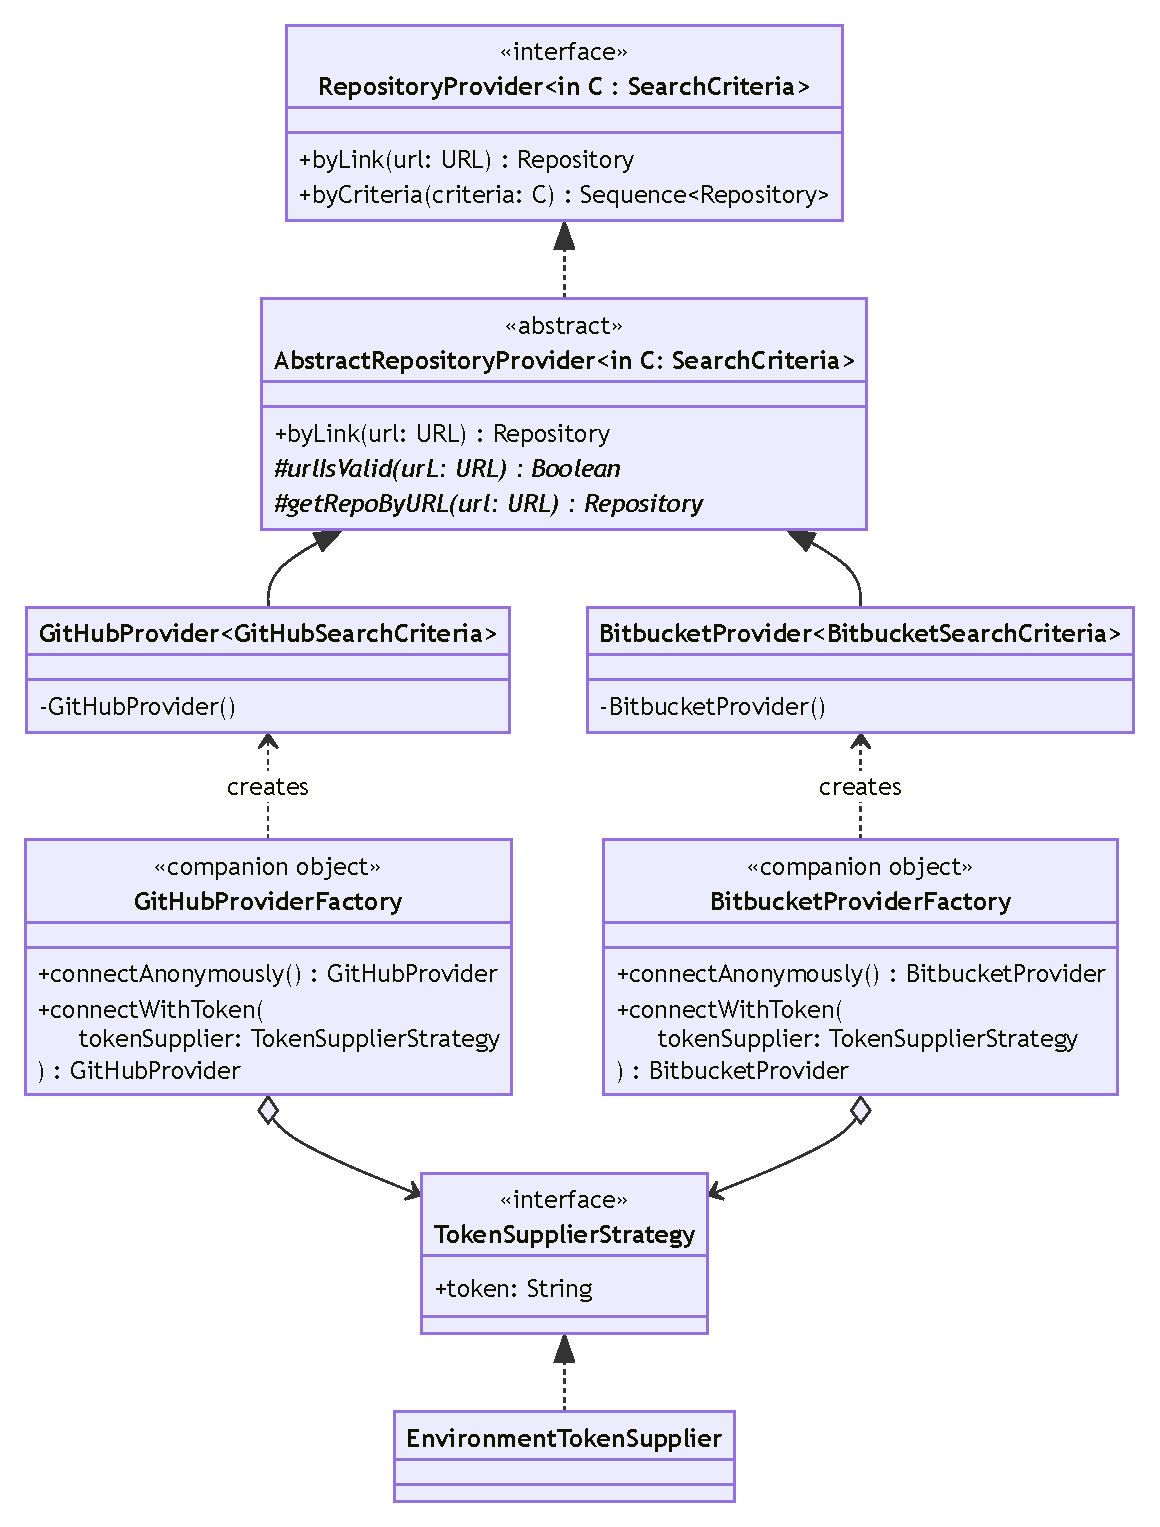
\includegraphics[width=0.9\textwidth]{resources/img/02-provider.pdf}
    \caption{Schema UML dei provider.}
    \label{img:02-provider}
\end{figure}

Viste le limitazioni in termini di numero di richieste che i due servizi impongono \footnote{Sia \textit{GitHub} che \textit{Bitbuckt} hanno un limite massimo di richieste che possono essere effettuate in un certo intervallo di tempo che varia in base la richiesta sia autenticata o meno. Questi vincoli sono imposti per garantire la protezione da attacchi di tipo \textit{Denial of Service}, consentire la scalabilità e garantire buone prestazioni in termini di tempo di risposta.} e la conseguente necessità di autenticarsi mediante degli opportuni \textit{token} per effettuare le richieste \textit{REST}, si è optato di demandare la logica di recupero dei suddetti \textit{token} di autenticazione all'interfaccia \texttt{TokenSupplierStrategy} che reifica il \textit{pattern} \textit{Strategy} \cite{gof}.
%
L'implementazione di \textit{default} ricerca tra variabili d'ambiente, ma altri approcci possono essere introdotti in modo del tutto trasparente ai \textit{provider}.

La creazione dei \textit{provider} avviene per mezzo di due \textit{static factory} \cite{effective-java}, incapsulate all'interno dei due \textit{provider}, in modo da permettere di ottenere un oggetto \textit{provider} anche senza autenticazione.
%
Nonostante questo sia in genere sconsigliato per via delle limitazioni sopra citate, può essere utile in fase di \textit{testing} per permettere di testare il sistema anche in contesti in cui non sia possibile usare \textit{token} di autenticazione validi, ad esempio nel contesto delle \textit{GitHub Actions} nei \textit{workflow} scatenati da eventi di tipo \textit{Pull Request} (vedi...\todo{ref al capitolo implementazione, paragrafo CI})

Dopo una prima analisi delle \textit{API} dei due servizi di \textit{hosting} si è convenuto di permettere di recuperare i progetti mediante due metodi: un \textit{link} diretto alla \textit{repository}, oppure mediante un criterio di ricerca, rappresentato dall'interfaccia \texttt{SearchCriteria}.
%
Per permettere che questi siano componibili è stato qui utilizzato il pattern \textit{Decorator} \cite{gof}.
%
La classe astratta che funge da decoratore è \texttt{(GitHub|BitBucket)CompoundCriteria} e le sue concrete implementazioni permettono di specificare il nome della \textit{repository} o il linguaggio.
%
In questo modo possono essere creati dinamicamente criteri compositi in base alle esigenze del \textit{client} e in futuro potrebbero essere aggiunti nuovi criteri di ricerca, come il numero di stelle ricevute, il \textit{topic} piuttosto che la data di creazione, aderendo all'\textit{Open Closed Principle} secondo cui le entità di un sistema devono essere aperte all'estensione, ma chiuse alla modifica.
%
Il \textit{design} è presentato in \Cref{img:02-search-criteria}.

\begin{sidewaysfigure}
    \centering
    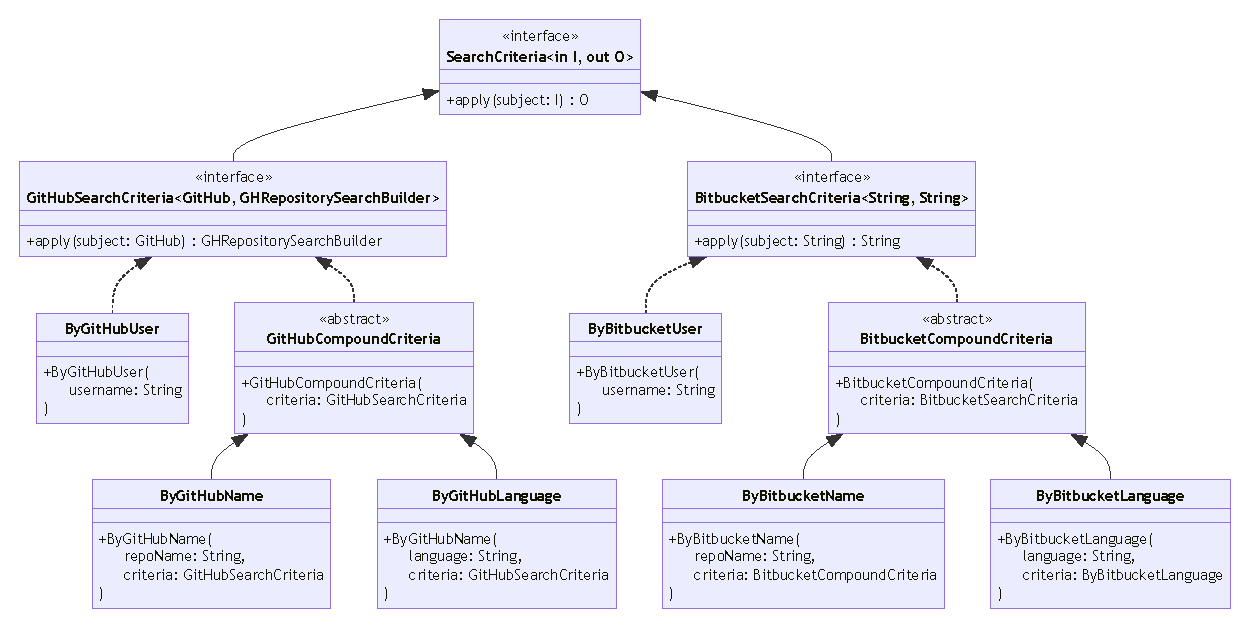
\includegraphics[width=\textwidth]{resources/img/02-search-criteria.pdf}
    \caption{Schema UML dei criteri di ricerca delle \textit{repository}.}
    \label{img:02-search-criteria}
\end{sidewaysfigure}

Le \textit{repository} sono modellate attraverso l'omonima interfaccia, le cui concrete implementazioni rappresentano degli \textit{Adapter} \cite{gof} alle interfacce di libreria utilizzate.
%
Questo permette di essere indipendenti dalla specifica libreria utilizzata, che rimane un dettaglio implementativo, e avere un livello di astrazione adeguato al contesto applicativo.
%
Per quanto attiene la logica del recupero dei sorgenti, in pieno accordo con il \textit{Single Responsability Principle}, è demandata a \texttt{RepoContentSupplierStrategy}.
%
La strategia attualmente in uso consiste nell'effettuare il \textit{clone} della repository in una cartella in locale.

\begin{figure}[h!]
    \makebox[\textwidth][c]{
        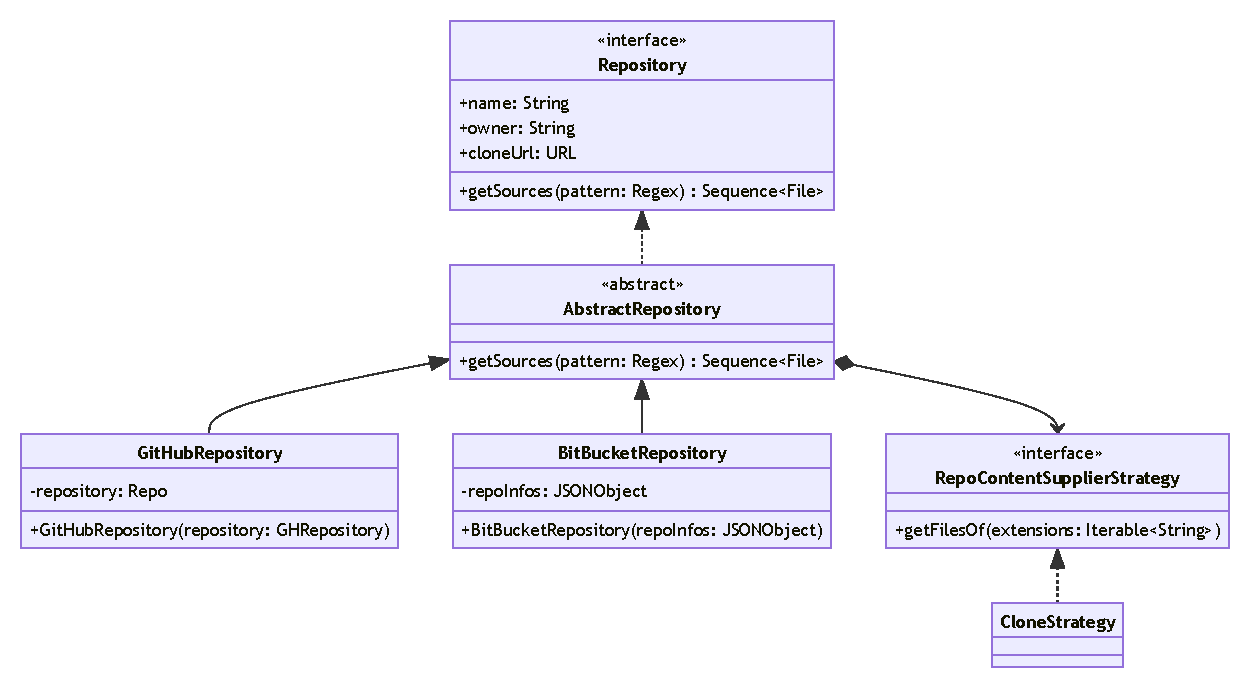
\includegraphics[width=1.2\textwidth]{resources/img/02-repos.pdf}
    }
    \caption{Schema UML delle repository.}
    \label{img:02-repos}
\end{figure}

\subsubsection*{Analizzatore e \textit{detector}}
L'analizzatore, il \textit{filter} e il \textit{detector} sono il cuore dell'intero sistema.
%
Il loro \textit{design} è stato pensato in modo tale da permettere il massimo grado di configurabilità e di estendibilità.
%
Presumibilmente, infatti, questi sono i componenti che varieranno più spesso nell'arco del ciclo di vita di questo \textit{software} e il cui grado di configurabilità influirà certamentente in modo preponderante sia sulle prestazioni, sia sull'efficacia del sistema.

Tutti e tre i componenti sono stati progettati, in stile funzionale, come delle funzioni che, preso i \textit{input} uno più argomenti, ritornano in \textit{output} l'\textit{input} del componente successivo:.
%
L'esecuzione di una tecnica è, infatti, una catena di funzioni applicate in sequenza.

L'analizzatore è il componente che si occupa di trasformare i file sorgenti in rappresentazioni confrontabili.
%
Indipendentemente dalla tipologia di analisi che si voglia applicare, la trasformazione non avviene tramite un semplice passaggio, bensì una sequenza di operazioni che sono eseguite sequenzialmente in cascata.
%
Nel caso in esame, queste sono: il \textit{parsing} del file, una fase di \textit{preprocessing} ed infine la \textit{tokenizzazione} del sorgente.
%
Questa sequenza di azioni è naturalmente modellata attraverso il pattern \textit{Pipeline} \cite{pipeline-pattern}: ogni singolo stadio è modellato attraverso l'interfaccia \texttt{StepHandler} e la \textit{pipeline} viene costruita all'interno del concreto \texttt{Analyzer}, nel nostro caso \texttt{JavaTokenizationAnalyzer}.

\begin{figure}[h!]
    \centering
    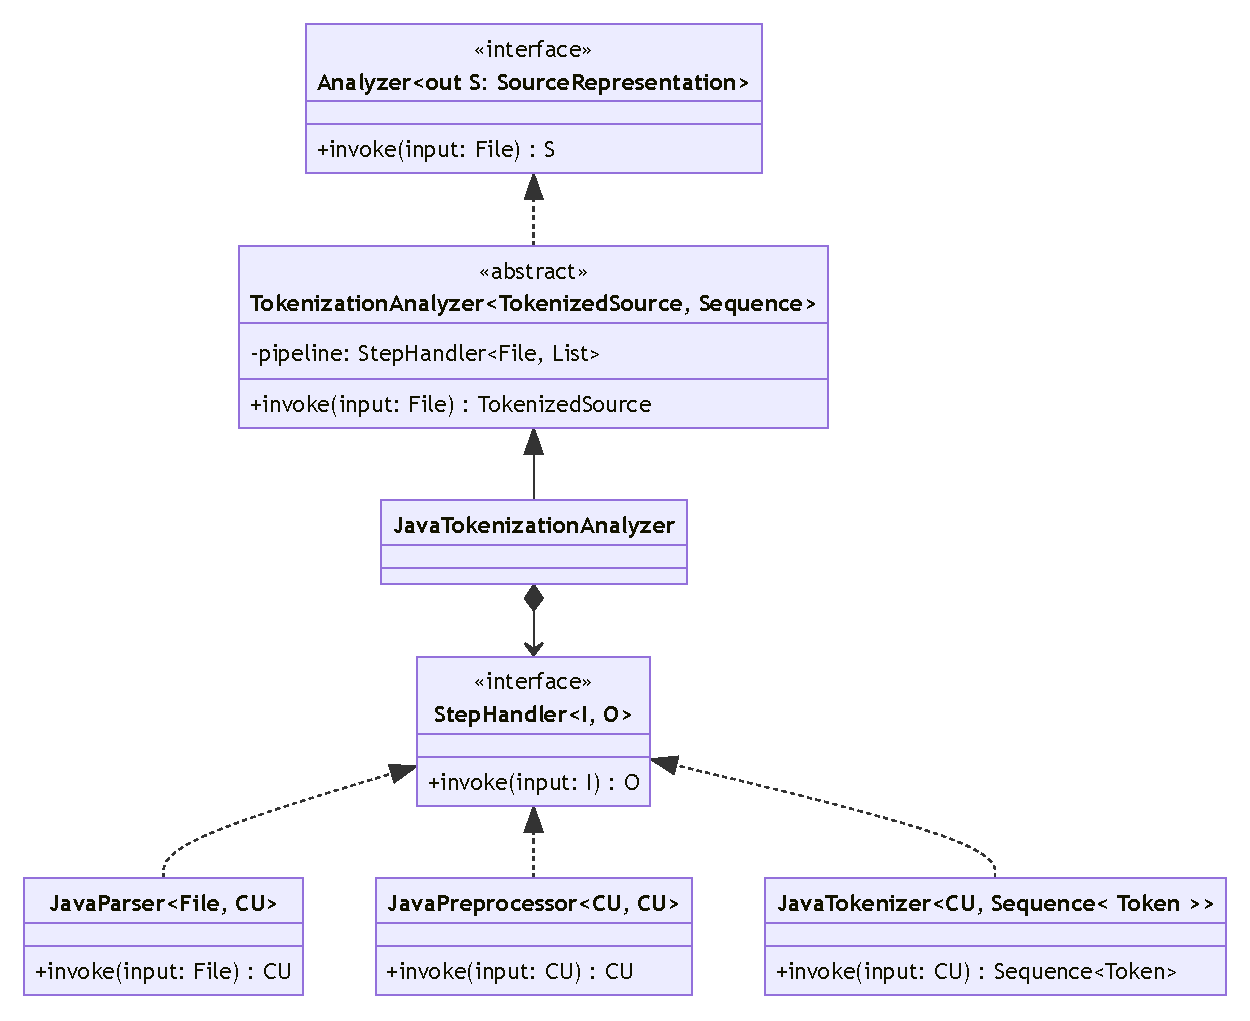
\includegraphics[width=\textwidth]{resources/img/02-analyzer.pdf}
    \caption{Schema UML dell'analizzatore.}
    \label{img:02-analyzer}
\end{figure}

La rappresentazione intermedia prodotta dall'analizzatore è modellata dall'interfaccia \texttt{SourceRepresentation} (\Cref{img:02-representations}). 
%
Tra tutte, quella implementata nell'attuale sistema è composta da una sequenza di \textit{token} e perciò denominata \texttt{TokenizedSource}.
%
L'elenco dei possibili tipi di \textit{token} che la compongono dipende chiaramente dal linguaggio utilizzato.
%
La strategia di recupero di questi ultimi è affidata, al solito tramite \textit{Strategy}, all'interfaccia \texttt{TokenTypesSupplier}, la cui implementazione di \textit{default} effettua la de-serializzazione di un file di configurazione in cui sono salvati tutti le tipologie di \textit{token}.

\begin{figure}[h!]
    \centering
    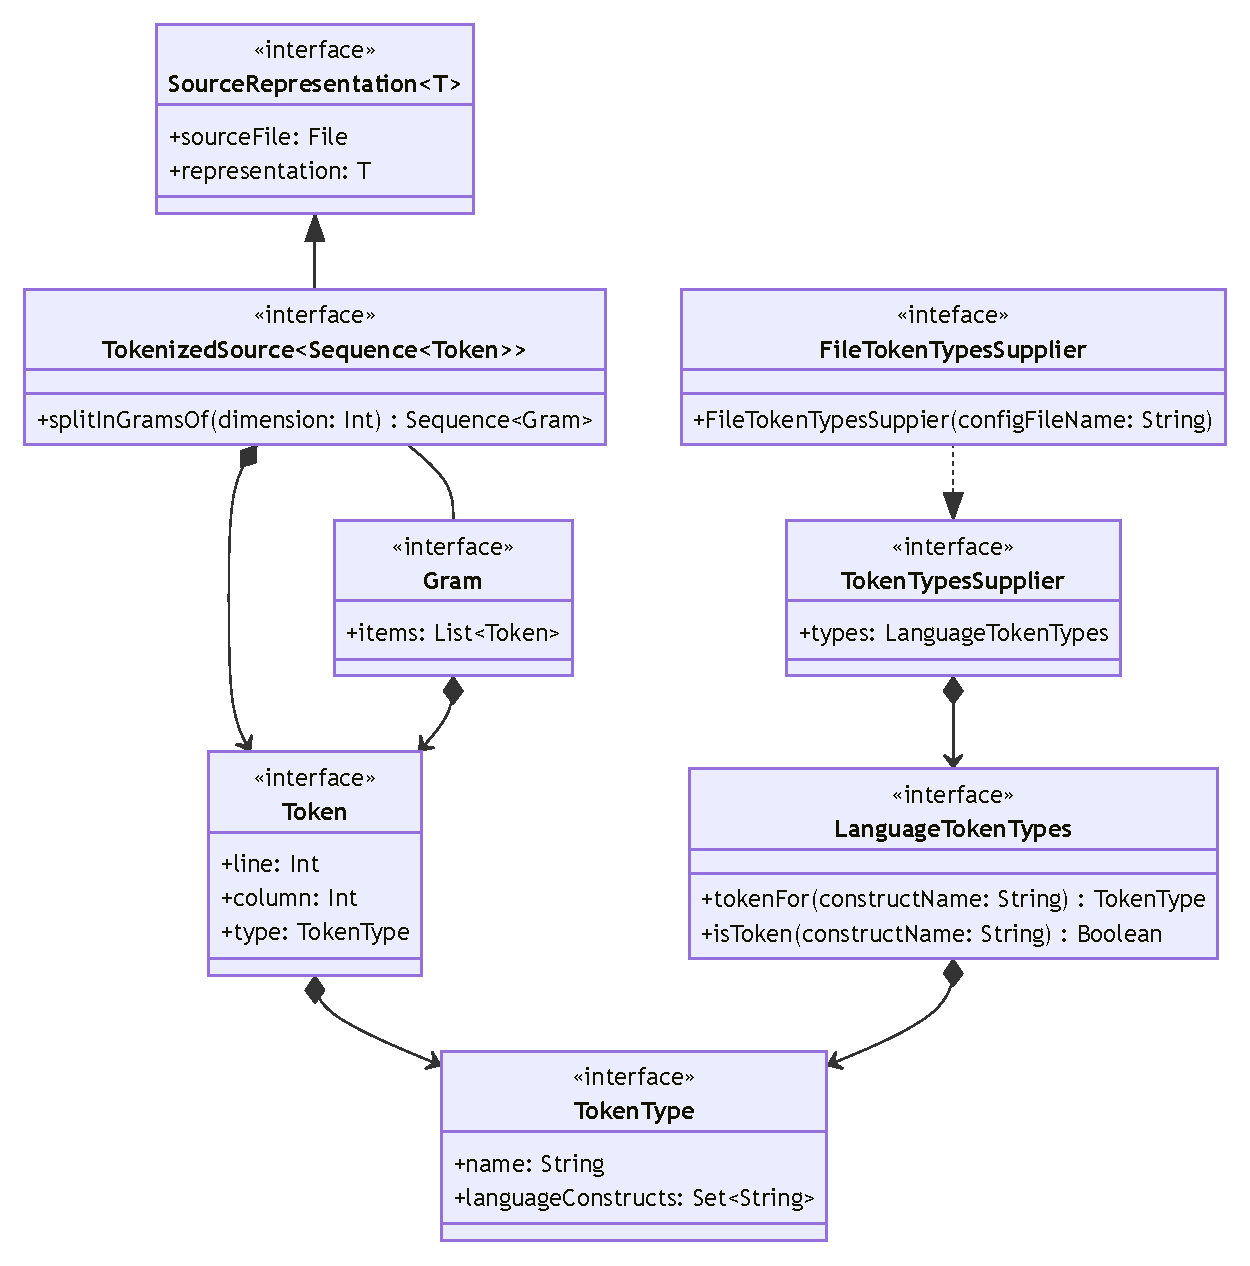
\includegraphics[width=\textwidth]{resources/img/02-representations.pdf}
    \caption{Schema UML delle rappresentazioni intermedie.}
    \label{img:02-representations}
\end{figure}

Le rappresentazioni generate dal processo di analisi, vengono poi opportunamente filtrate per mezzo di un \texttt{RepresentationFilter} che, preso in \textit{input} una istanza dell'insieme delle \textit{submission} e l'insieme del \textit{corpus} con cui confrontarla, ne effettua un filtraggio secondo opportune metriche.
%
Per farlo, fa uso di un \texttt{Indexer} che crea, a partire dalle rappresentazioni, indici (strutture dati) su cui poter effettuare analisi \dots

\todo{filter + schema}

\texttt{PlagiarismDetector} rappresenta invece il componente che individua le similarità tra una coppia di \texttt{SourceRepresentation} e si occupa di calcolare la loro similarità.
%
Poiché vi sono una molteplicità di algoritmi presenti in letteratura che assolvono a questo compito, si è deciso d'implementarli sotto forma di gerarchia di classi di algoritmi il cui contratto comune è definito da \texttt{ComparisonStrategy}. 
%
In particolare, ogni classe implementante \texttt{ComparisonStrategy} genera un \texttt{Match}, dove per \texttt{Match} si intende due sezioni simili di \textit{SourceRepresentation}.
%
L'insieme dei \texttt{Match} che compongono la comparazione di due \texttt{SourceRepresentation} sono raggruppate in un \texttt{ComparisonResult}, il cui grado di similarità è stimato dalla \texttt{SimilarityEstimationStrategy}.

Applicato alla tecnica di \textit{tokenizzazione}, i due concreti algoritmi che implementano la \textit{detection} sono \texttt{Greedy String Tiling} e \texttt{RKRGreedyStringTiling} che ne rappresenta un'estensione più performante.
%
Entrambi generano dei \texttt{TokenMatch}. \dots

\begin{sidewaysfigure}
    \centering
    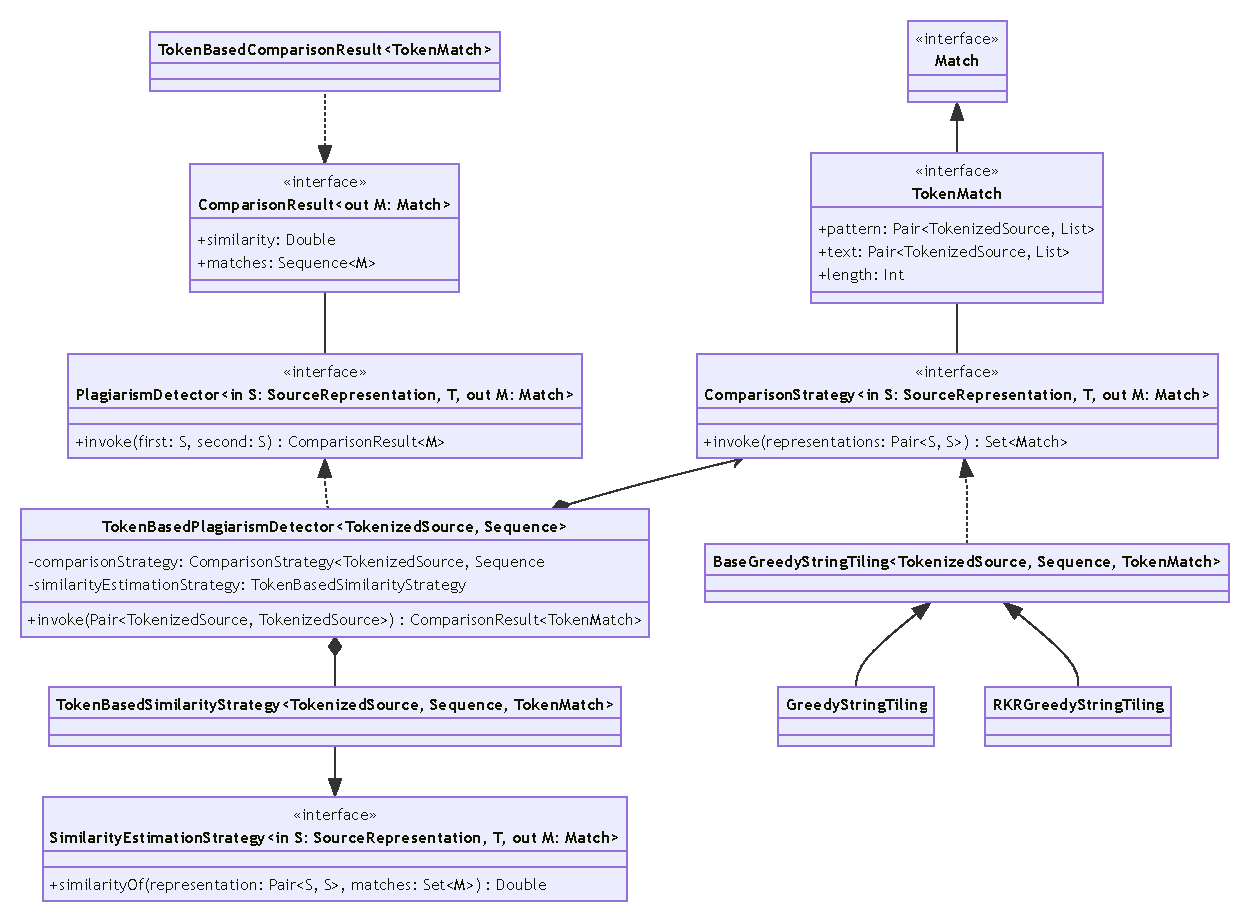
\includegraphics[width=\textwidth]{resources/img/02-detector.pdf}
    \caption{Schema UML del \textit{detector}.}
    \label{img:02-detector}
\end{sidewaysfigure}

Tutti e tre i componenti, \texttt{Analyzer}, \texttt{Filter} e \texttt{PlagiarismDetector}, sono incapsulati all'interno di un concreto \texttt{TechniqueFacade} \cite{gof}.
%
Si è deciso di adottare questo approccio principalmente per due motivi:
\begin{itemize}
    \item la specifiche strategie di analisi e di confronto devono essere istanziate e opportunamente configurate a \textit{runtime} a seconda del tipo di tecnica e delle opzioni scelte dall'utente. Inoltre, devono essere coerenti tra loro: non è possibile, ad esempio, poter istanziare un analizzatore per effettuare la \textit{tokenizzazione} e un rilevatore che non operi sulla sequenza di \textit{token}. Il \textit{facade} pertanto si occupa d'istanziare i corretti componenti necessari all'esecuzione della tecnica in accordo con i parametri a lui fornitogli, sollevando il \textit{client} da questa responsabilità.
    \item Il processo di analisi e confronto può essere complesso. Pertanto si fornisce ai \textit{client} un'interfaccia semplificata che assolve al compito di eseguire una generica tecnica, rendendo di fatto trasparente al chiamante la complessità del sottosistema che, dal suo punto di vista, è di fatto una \textit{black box}.
\end{itemize}

Come già detto, l'aspetto della configurabilità è un aspetto molto importante in questo contesto, in quanto la scelta dei parametri influisce sull'efficacia del rilevamento.
%
In particolare, una specifica sessione è legata ad una particolare configurazione (\texttt{RunConfiguration}) che contiene tutte le informazioni necessarie per l'esecuzione, tra cui la tecnica da utilizzare, l'insieme delle \textit{repository} che compongono la \textit{submission} e quelle del \textit{corpus}, nonché il concreto \texttt{ReportsExporter} a cui è affidata l'esportazione dei \textit{report} generati.
%
Tale configurazione è creata da un concreto \texttt{RunConfigurator}: i due metodi supportati, alternativi tra loro, sono il \texttt{CLIConfigurator} che crea la configurazione a partire dagli argomenti da riga di comando, oppure il \texttt{FileConfigurator} che sfrutta un file di configurazione per impostare tutti i parametri.
%
Nulla vieta che in un prossimo futuro, se si volesse dare una veste grafica al sistema, si possa implementare una interfaccia che specializza \texttt{RunConfigurator} e che viene implementata dalla o dalle classi che si occupano di creare le componenti grafiche.

In \Cref{img:02-session} è mostrato lo schema UML delle classi che mostra i rapporti 

\todo{schema sequenza}

\begin{sidewaysfigure}
    \centering
    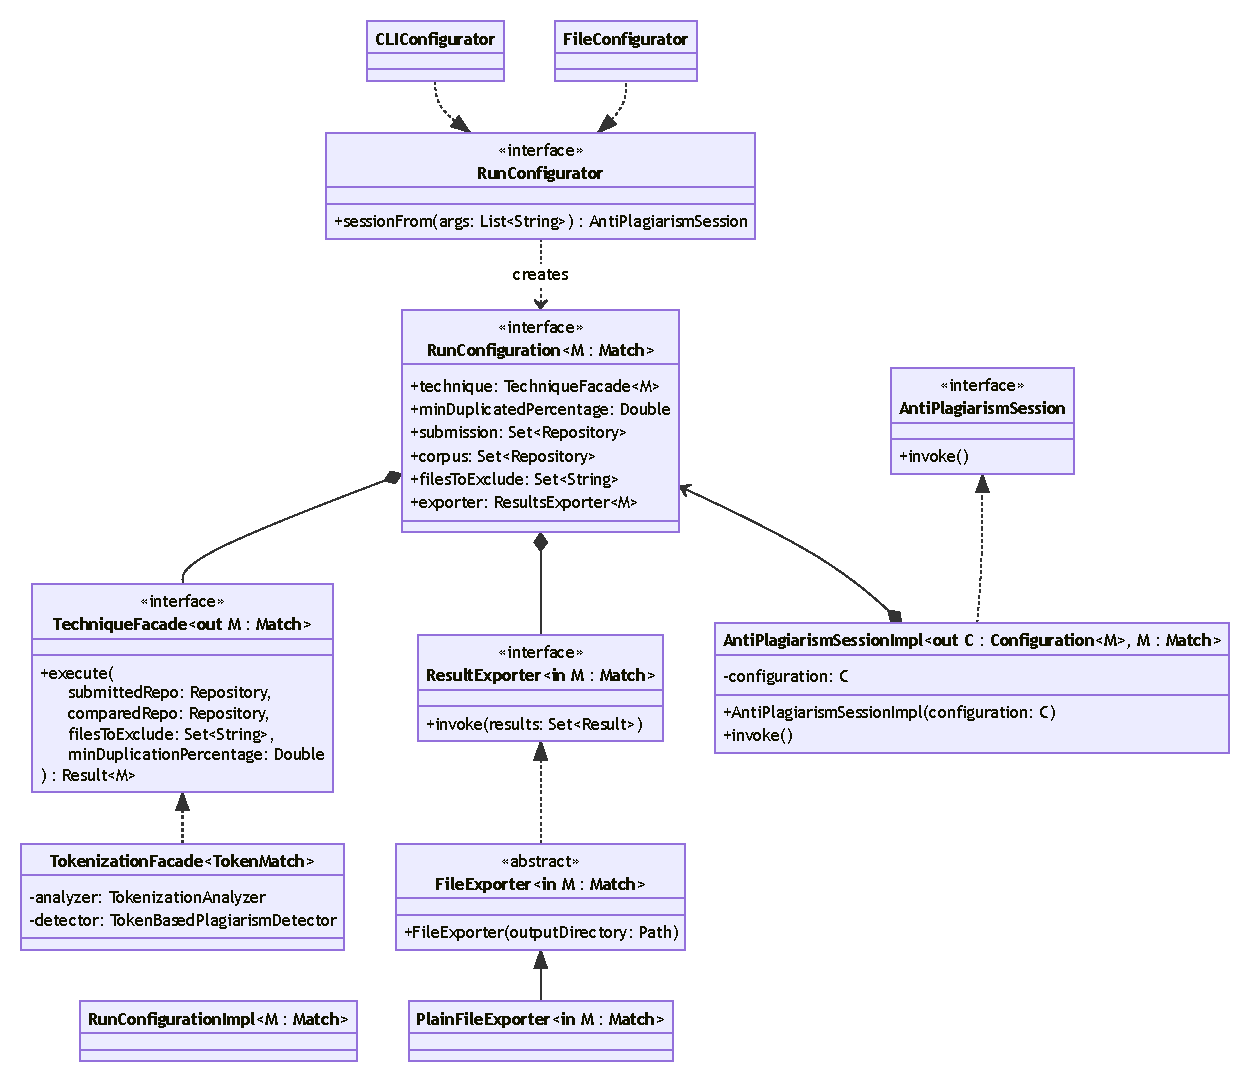
\includegraphics[width=0.9\textheight]{resources/img/02-session.pdf}
    \caption{Schema UML della sessione}
    \label{img:02-session}
\end{sidewaysfigure}

\todo{caching}

	% ! TeX root = ../../thesis.tex
\chapter{Implementazione}
\label{chapter:implementation}
In questo capitolo vengono affrontati gli aspetti implementativi del sistema, descrivendo le tecnologie e i paradigmi utilizzati.

\vspace*{0.5cm}

La tecnica impiegata nel sistema appartiene alla famiglia di tecniche \textit{structure-based} e si compone macroscopicamente di tre fasi, schematizzate in \Cref{img:03-system-overview}:
\begin{enumerate}
	\item \textbf{Analisi}: i sorgenti sono \textit{parsati}, preprocessati e \textit{tokenizzati};
	\item Una fase opzionale di \textbf{filtraggio};
	\item \textbf{Rilevamento} delle somiglianze.
\end{enumerate}

\begin{figure}[h!]
    \centering
    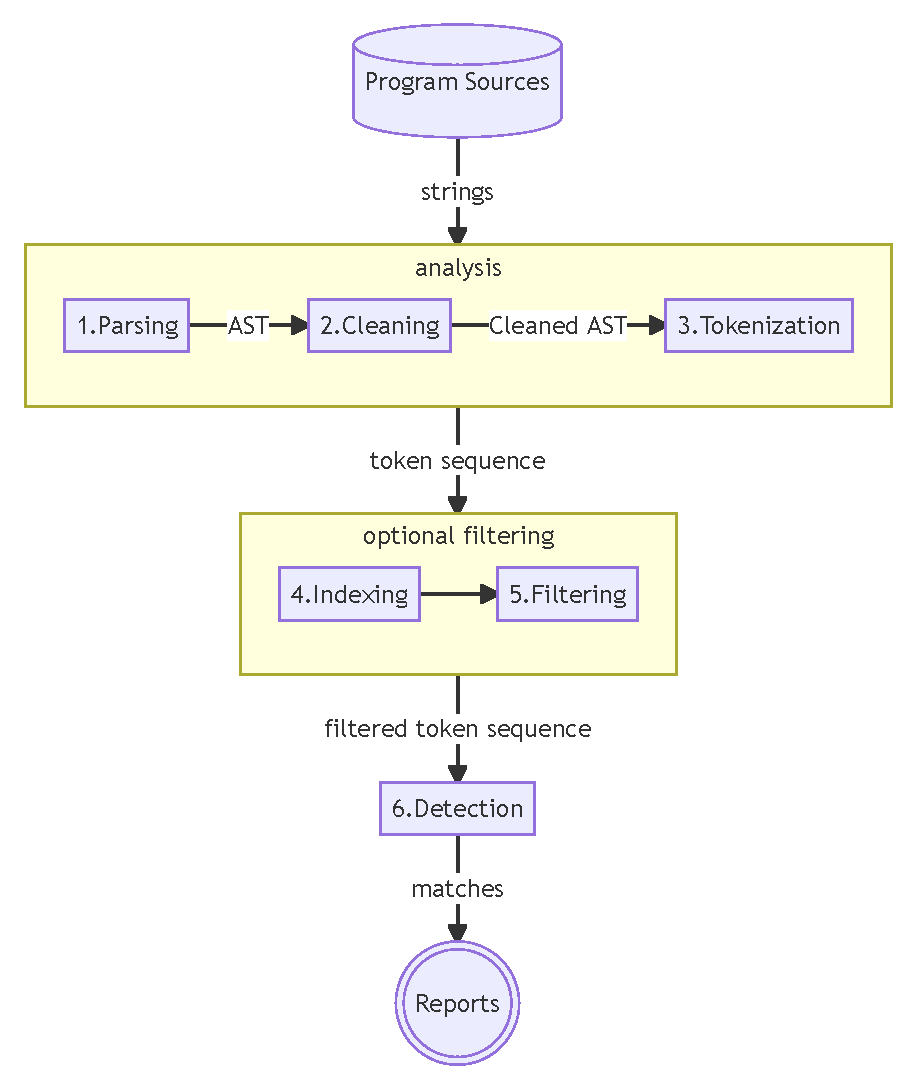
\includegraphics[width=0.8\textwidth]{resources/img/03-system-overview.pdf}
    \caption{Visione d'insieme delle fasi della tecnica impiegata.}
    \label{img:03-system-overview}
\end{figure}

Di seguito ciascuna delle tre viene approfondita.

\section{Tecnica di analisi}
Il primo passo consiste nell'effettuare il \textit{parsing} dei sorgenti, affidato alla libreria JavaParser\footnote{\url{https://javaparser.org/}}.
%
JavaParser è una libreria \textit{open source} che permette di effettuare il \textit{parsing} di sorgenti scritti in linguaggio Java, fornendo comodi meccanismi per l'analisi e la manipolazione degli stessi.

Il risultato del \textit{parsing} è un albero sintattico equivalente a quello mostrato in \Cref{img:01-ast} che rappresenta la struttura dei sorgenti.

Tuttavia, nonostante la generazione dell'albero sintattico sollevi dalla responsabilità di eliminare dal sorgente \textit{token} superflui, come gli spazi e i punti e virgola, in quanto naturalmente modellati dalla struttura stessa dell'albero, tale AST contiene ancora informazioni sovrabbondanti, come le dichiarazioni di \texttt{import} e dei \texttt{package}.
%
Per questo motivo è necessario una fase intermedia di \textit{preprocessing} in cui l'albero viene “sfoltito”. In particolare, in questa fase l'albero viene visitato e, oltre a rimuove le dichiarazioni suddette, sono rimosse anche le funzioni \texttt{hashCode()}, \texttt{equals()} e \texttt{toString()}.
%
Queste, infatti, nella maggioranza dei casi, vengono automaticamente generate dall'\textit{IDE} e non sono rappresentative della logica dei sorgenti.

A seguire avviene la conversione del codice sorgente in una sequenza di \textit{token}.
%
Si noti che la fase di \textit{tokenizzazione} vera e propria descritta nella \Cref{01-tokenization} è già stata eseguita internamente dal \textit{parser} di JavaParser i cui \textit{token} sono quelli presenti nell'albero.
%
Tali \textit{token}, tuttavia, rappresentano in modo molto specifico la struttura del programma: ad ogni tipo del linguaggio è associato un tipo differente di \textit{token}.
%
Come descritto nella \Cref{01-tokenization} l'obiettivo è creare invece un insieme di \textit{token} "lasco" che raggruppi tipi di \textit{token} equivalenti a livello semantico.

A questo scopo, l'albero sintattico preprocessato viene visitato e, per ogni nodo, si emette un \textit{token}, con le relative informazioni circa la sua posizione nel sorgente, a seconda sia una dichiarazione semanticamente rilevante o meno.

In particolare, è stato costruito un file di configurazione \textit{Yaml}\footnote{Linguaggio, \textit{superset} di Json, per la serializzazione di dati che viene impiegato per la scrittura di file di configurazione: \url{https://yaml.org/}.} (\Cref{lst:token-config-file}) in cui sono elencati i tipi di dichiarazioni rilevanti, eventualmente tralasciando tipi troppo dettagliati, come \texttt{PrimitiveType} o \texttt{VarType}, ed aggregando tra loro dichiarazione semanticamente simili e che potrebbero essere facilmente cambiate per offuscare la copiatura.
%
Ad esempio, sono state aggregate sotto un unico tipo \texttt{loop-stmt} tutti i costrutti che effettuano un ciclo.
%
In questo modo un cambio sintattico di tipo non sarà sufficiente ad aggirare il sistema perché verrà generato lo stesso tipo di \textit{token}.
%
Si noti che questo approccio è molto flessibile e può essere "aggiustato" a piacimento nel caso sia necessario effettuare una \textit{tokenizzazione} con un insieme di \textit{token} più stringente.

\lstinputlisting[
 	language=yaml,
 	caption={Porzione del file di configurazione con la definizione dei tipi di \textit{token}},
 	label={lst:token-config-file},
]{resources/code/03-token-types.yml}

Il risultato dell'applicazione del processo sopra descritto al \Cref{lst:test-analysis} viene presentato nel \Cref{lst:result-tokenization}

\lstinputlisting[
 	caption={Risultato dell'analisi del \Cref{lst:test-analysis}},
 	label={lst:result-tokenization},
]{resources/code/03-AnalyzedTestAnalysis}

% vengono anche tolti i duplicati :)

%-----------------------------------------------------------------------------
\section{Filtraggio}
\label{03:filtering-phase}
%-----------------------------------------------------------------------------
A seguito dell'analisi del codice sorgente e della generazione della sequenza di \textit{token} i sorgenti del \textit{corpus} possono essere filtrati, al fine di limitare il numero di progetti da dover confrontare.
%
Questo \textit{step} rappresenta uno snodo critico nella \textit{pipeline} di azioni da eseguire in quanto scambia una frazione dell'efficacia del sistema in favore dell'efficienza: una stima fuorviante della similarità di una coppia di progetti può comportare l'esclusione dalla comparazione degli stessi, con la conseguente perdita di sensibilità nel caso in cui rappresentassero dei veri casi di copiatura.
%
Per questo motivo la fase di filtraggio è \textit{opzionalmente} eseguita a discrezione dell'utente, che si presume possa valutare se necessita di un'analisi più veloce ma meno esaustiva o viceversa.

Come già presentato nella \Cref{01-tokenization}, il processo di filtraggio è preceduto da una fase d'indicizzazione in cui vengono aggregati i dati sotto forma di una struttura dati per mezzo della quale è possibile estrarre informazioni statistiche significative per la stima della similarità.

Nel sistema è attualmente implementato un indice equivalente a quello presentato in \Cref{table:token-indexing} a partire dal quale la similarità tra progetti è stata calcolata mediante la \textbf{similarità coseno}.
%
Essa è una metrica euristica ampiamente utilizzata nel contesto dell'analisi testuale che misura la similitudine di due vettori calcolando il coseno del loro angolo: 
\begin{equation}
	cosine\_similarity(A,B) = \frac{A \cdot B}{||A|| ||B||} 
		= \frac{\sum_{k=1}^{n} A(k) B(k)}{\sqrt{\sum_{k=1}^{n}A(k)^2 \cdot \sum_{k=1}^{n} B(k)^2}}
\end{equation}
dove $A$ e $B$ sono due vettori di attributi numerici a $n$ dimensioni.

In generale, il risultato della similarità è un valore compreso tra $-1$ e $1$ dove $-1$ indica che i due vettori sono \textit{anti}-correlati (hanno verso opposto), $1$ indica massima correlazione e $0$ un'assenza di correlazione (i due vettori sono ortogonali tra loro).

Nel nostro caso, il contenuto dei due vettori è la frequenza dei tipi di \textit{token} in cui il $k$-esimo elemento contiene il numero di volte in cui il $k$-esimo tipo di \textit{token} ricorre nel sorgente, oppure $0$ se non presente.
%
Poiché le frequenze sono valori sempre positivi, nel caso in esame, si otterranno valori compresi tra $0$ e $1$, dove $1$ indica che i tipi di \textit{token} contenuti nelle due rappresentazioni sono gli stessi, presenti in egual numero ma non necessariamente disposti nello stesso ordine, e $0$ indica che non c'è alcun tipo di \textit{token} comune.

A seguito della stima della similarità coseno, tutte le coppie di rappresentazioni la cui similarità è inferiore a un valore di soglia sono esclusi.
%
Tale valore è calcolato, seguendo quanto riportato in \cite{es-plag}, utilizzando la formula riportata nell'\Cref{eq:cosine-filtering-threshold}.

\begin{equation}
\label{eq:cosine-filtering-threshold}	
	threshold = sim_{min} + init\_threshold \cdot (sim_{max} - sim_{min})
\end{equation}

dove $init\_threshold$ è un valore compreso tra $0$ e $1$ (corrispondente al range $0-100\%$) e $sim_{max}$ e $sim_{min}$ sono rispettivamente la similarità coseno massima e minima risultante dalla comparazione di tutte le coppie.

Secondo le valutazioni presentate in \cite{es-plag} questo tipo di filtraggio aumenta l'efficienza del sistema con un compromesso in termini di efficacia che rimane accettabile fintanto che la soglia $init\_threshold$ è mantenuta al di sotto del 60\%.

\section{Rilevamento delle somiglianze}
\label{03-matching-algorithms}
Gli algoritmi impiegati per confrontare due sequenze di \textit{token} sono il \textit{Greedy String Tiling} e il \textit{Running Karp-Rabin Greedy String Tiling}, che ne rappresenta una sua evoluzione, introdotti da M. Wise nel 1993 in \cite{wise-running-93} a seguito della necessità di sviluppare proprio un sistema automatico antiplagio, anche se negli anni successivi gli stessi algoritmi sono stati impiegati in altri campi, tra cui il confronto di sequenze di proteine/DNA.

Sebbene questi siano stati concepiti per lavorare su sequenze di stringhe, possono essere facilmente riadattati per operare su sequenze di \textit{token}

Dette $A$ e $B$ due sequenze di \textit{token}, un algoritmo per misurare la similarità in questo dominio deve determinare una sottosequenza comune che abbia le seguenti proprietà:
\begin{itemize}
	\item ogni \textit{token} di $A$ può essere abbinato solo con esattamente un solo \textit{token} di $B$;
	\item le sottosequenze comuni devono essere trovate indipendentemente dalla loro posizione nel sorgente;
	\item le sottosequenze più lunghe sono preferite a quelle più piccole, in quanto le sottosequenze brevi è molto probabile rappresentino casi spuri.
\end{itemize}

L'algoritmo si compone principalmente di due fasi:
\begin{itemize}
	\item \textbf{Fase 1}: in questa fase, viene ricercata la corrispondenza più lunga. Questo è fatto grazie un triplo ciclo innestato: il primo itera sui token della sequenza più corta, denominata \textit{pattern}, il secondo compara ciascuno di questi con ogni \textit{token} della sequenza più lunga, denominata \textit{text}. Se i due \textit{token} corrispondono il ciclo più interno cerca di estendere il \textit{match} il più possibile (fermandosi non appena trova un \textit{token} che nelle due sequenze differisce).

	\item \textbf{Fase 2}: questa fase marca ciascun \textit{match} di lunghezza massima (\textit{maximal match}) trovato nella fase precedente. Questo garantisce che ciascun \textit{token} venga usato per un solo \textit{match} e divenga indisponibile per i \textit{match} successivi (che hanno una minor lunghezza). Nella terminologia di \cite{wise-running-93} i \textit{match} i cui \textit{token} sono stati marcati sono denominati \textit{tile}. Si noti che, anche se un \textit{match} è parzialmente occluso e perciò non viene marcato, una versione più corta dello stesso \textit{match} può essere marcato durante le successive iterazioni.
\end{itemize}

Queste due fasi vengono ripetute fino a quando non vengono trovate più corrispondenze di lunghezza almeno \texttt{minimum\_match\_length}.
%
Tale valore è imposto per non generare troppe sequenze spurie di lunghezza irrisoria e garantire risultati migliori.
%
Giacché la lunghezza dei \textit{match} diminuisce ad ogni iterazione è garantito che l'algoritmo termini.

Lo pseudocodice dell'algoritmo è presentato nel \Cref{lst:gst}.

\lstinputlisting[
	language=pseudocode,
 	caption={Pseudocodice dell'algoritmo \textit{Greedy String Tiling (GST)}. In accordo con la terminologia del \textit{paper}, $P$ rappresenta il \textit{pattern}, ovvero la sequenza da confrontare più corta, mentre $T$ il \textit{text}, ovvero la sequenza tra le due più lunga.},
 	label={lst:gst},
]{resources/code/03-gst}

Questo algoritmo è dimostrato \cite{wise-running-93} essere ottimo in termini di massimizzazione della copertura delle stringhe.
%
Nonostante ciò, nel caso peggiore, ha una complessità $O(n^3)$ e pertanto è molto inefficiente.

Per far fronte a questo problema è stato ideato un nuovo algoritmo chiamato \textit{Running Karp Rabin Greedy String Tiling}.
%
L'idea su cui si fonda per velocizzare il confronto è impiegare una funzione di \textit{hashing}.
%
In particolare, il valore di \textit{hash} di ogni sottosequenza di lunghezza $s$ del \textit{pattern} viene confrontato con il valore di \textit{hash} di quelle del \textit{text}.
%
Laddove i due valori corrispondano, e solo in questo caso, le sottosequenze vengono confrontate \textit{token} per \textit{token} per assicurarsi che effettivamente siano uguali e non frutto di una collisione della funzione di \textit{hash}.

Nel \Cref{lst:rkr-scanpattern} viene mostrato lo pseudocodice della \textit{routine} che si occupa di effettuare questo confronto.
%
Come si può osservare, nelle righe 1-3 vengono calcolati i valori di \textit{hash} di tutte le sottosequenze (non marcate) di lunghezza $s$ del \textit{text} e vengono salvati in una \textit{hashtable}, una mappa con le corrispondenze sottosequenza di \textit{token}-valore di \textit{hash}.
%
Lo stesso viene fatto per il \textit{pattern} con la differenza che, non appena calcolato il valore \textit{hash} per la sottosequenza considerata, si verifica se lo stesso sia già presente nella \textit{hashtable}.
%
In questo caso, infatti, potrebbe effettivamente esserci una corrispondenza e si procede verificando \textit{token} per \textit{token}.
%
Si noti che nei casi in cui la corrispondenza sia effettiva e non sia causata da un artefatto della funzione di \textit{hash}, il \textit{match} è esteso fino al primo \textit{token} non corrispondente, proprio come nel precedente algoritmo.

\lstinputlisting[
 	language=pseudocode,
 	caption={Pseudocodice della \textit{routine} \texttt{scanpattern} dell'algoritmo \textit{RKR-GST}.},
 	label={lst:rkr-scanpattern},
]{resources/code/03-rkr-gst-scanpattern}

Nella versione originale dell'algoritmo la struttura dati utilizzata per memorizzare i \textit{match} è una lista di code in cui ogni coda memorizza i \textit{match} della stessa lunghezza, mantenuta ordinata per valori descrenti.

Il \Cref{lst:rkr-markarrays} presenta lo pseudocodice della \textit{routine} che effettua la marcatura dei \textit{match} individuati nella \textit{routine} \texttt{scanpattern}, corrispondente alla seconda fase dell'algoritmo precedente.
%
La principale differenza con la precedente versione risiede nel fatto che la marcatura viene effettuata per ogni \textit{match} e non solo per quelli di lunghezza massima.
%
Inoltre, se il \textit{match} risulta parzialmente occluso, ma la rimanente parte non occlusa è  di lunghezza $m \ge s$, questa viene salvata nella lista di code, in modo tale da essere valutata nella successiva iterazione in cui vengono valutati tutti i \textit{match} di lunghezza $m$ (righe 11-13).

\lstinputlisting[
 	language=pseudocode,
 	caption={Pseudocodice \textit{routine} \texttt{markarrays} dell'algoritmo \textit{RKR-GST}.},
 	label={lst:rkr-markarrays},
]{resources/code/03-rkr-gst-markarrays}

Infine, nel \Cref{lst:rkr-top-level} è mostrato l'\textit{entry-point} dell'algoritmo.
%
Come si può osservare, corrispondenze molto lunghe vengono trovate solo durante la prima iterazione: dopo di questa, infatti, non è possibile siano trovate corrispondenze maggiori del doppio della lunghezza di ricerca corrente.
%
Questo garantisce che, nelle successive iterazioni, l'algoritmo termini.

\lstinputlisting[
 	language=pseudocode,
 	caption={\textit{Entry-point} dell'algoritmo \textit{RKR-GST}.},
 	label={lst:rkr-top-level},
]{resources/code/03-rkr-gst-top-algorithm}

Il valore di $s$ (l'equivalente di \texttt{minimum\_match\_length} nell'algoritmo \textit{GST}) è scelto in modo tale da garantire che non vengano cercate corrispondenze troppo piccole.
%
Un valore plausibile di $s$ consigliato in \cite{wise-running-93} è 20.

Sebbene la complessità di questo algoritmo sia dimostrato essere, nel caso peggiore, $O(n^2)$, nel caso medio la complessità è pressoché \textbf{lineare}.
%
Ciò migliora notevolmente le prestazioni rispetto all'algoritmo \textit{Greedy String Tiling}.

\section{Stima della similarità}

\subsection*{Similarità tra coppie di sorgenti}
La misura della similarità di due sorgenti dovrebbe intuitivamente riflettere la frazione di \textit{token} dei programmi originali che sono "coperti" da \textit{match}.
%
Seguendo questo principio ci sono due possibili scelte che possono essere intraprese e che determinano la formula di stima di similarità: se si vuole che la similarità del 100\% significhi che le due sequenze sono identiche dobbiamo considerare entrambe le stringhe nel computo, come segue:
%
\begin{equation}
\label{eq:avg-norm-sim}
	sim_S(A, B) = \frac{2 \cdot \sum_{match \in tiles} length}{|A|+|B|}
\end{equation}
%
Se, invece, preferiamo che ogni programma che è stato copiato completamente (e poi magari esteso) produca una similarità del 100\%, dobbiamo considerare solo la sottosequenza più corta:
%
\begin{equation}
\label{eq:max-norm-sim}
	sim_S(A, B) = \frac{\sum_{match \in tiles} length}{min(|A|, |B|)}
\end{equation} 

Per mitigare il problema dell'insensibilità al riordino delle sottosequenze di cui è intrinsicamente affetta la tecnica di analisi impiegata, in \cite{es-plag} viene proposto di modificare la formula di stima della similarità introducendo un meccanismo di penalità ispirato dal principio che, solitamente, un numero elevato di sottosequenze comuni si verifica proprio a causa del riordino delle stesse. 
%
Applicando pertanto una penalità proporzionata al numero di sottosequenze comuni, maggiore sarà il numero di sottosequenze individuate, minore sarà il grado di similarità determinato.
%
Le formule aggiornate sono di seguito presentate.

\begin{equation}
	sim_S(A, B) = \frac{2 \cdot \bigl( \sum_{match \in tiles} length - (|tiles|-1) \bigr)}{|A|+|B|}
\end{equation}

\begin{equation}
	sim_S(A, B) = \frac{\sum_{match \in tiles} length - (|tiles|-1)}{min(|A|, |B|)}
\end{equation} 

\subsection*{Similarità tra coppie di progetti}
Vista la grande quantità di progetti di cui si dispone, sebbene i risultati ottenuti siano filtrati per non riportare singole coppie di sorgenti con una similarità inferiore a una soglia (scelta dall'utente), la quantità di risultati rimane corposa.
%
Pertanto, non è sufficiente stimare la similarità sorgente per sorgente, ma è necessario fornire una stima aggregata delle similarità progetto per progetto, così da individuare più facilmente, a un livello di granularità maggiore, i progetti simili.

In generale, questa stima di similarità è inferita a partire da quelle tra sorgenti come segue:

\begin{equation}
	\begin{split}
		sim_P(A, B) &= \underbrace{max \biggl\{ \frac{|\textit{sorgenti segnalati di A}|}{|\textit{sorgenti di A}|}, \frac{|\textit{sorgenti segnalati di B}|}{|\textit{sorgenti di B}|} \biggr\}}_\text{I} \\
		&  \cdot \underbrace{P_{75}(\textit{similarità sorgenti segnalati})}_\text{II}
	\end{split}
	\label{eq:project-similarity}
\end{equation}

dove $A$ e $B$ sono due progetti e $P_{75}$ il settantacinquesimo percentile (o terzo quartile) delle similarità dei sorgenti segnalati.

In questo modo, la seconda parte dell'equazione (II) fornisce una stima aggregata delle similarità dei sorgenti, considerando il valore di similarità che "lascia alla sua sinistra" il 75\% della distribuzione.
%
L'utilizzo di questa statistica è migliore della semplice media o mediana, in quanto queste darebbero stessa importanza a tutte le stime di similarità, fornendo risultati troppo bassi anche nei casi effettivi di copiatura, visto che, generalmente, anche in questi, vengono rintracciate sezioni con una bassa stima di similarità.

Tuttavia, applicare solo una statistica di aggregazione dei valori di similarità dei sorgenti segnalati può fornire misure fuorvianti nel caso in cui questi siano pochi (nell'ordine di alcune unità) ma con valori di similarità elevati.
%
Per questo motivo, la misura di similarità aggregata sopra descritta viene "pesata" sulla base del massimo rapporto tra $A$ e $B$ del numero di sorgenti segnalati e quelli del progetto in esame.
%
Così facendo, si andrà a diminuire il peso complessivo della similarità per quei progetti i cui sorgenti segnalati sono esegui rispetto alla loro totalità.
%
Questo determina tuttavia che copiature di circa il 50\% del progetto possano avere al più similarità 50\% nel caso limite in cui la II parte dell'\Cref{eq:project-similarity} sia uguale a 1.
%
Questo però è raro che accada perché significherebbe che le copiature sono frutto di un copia e incolla letterale; nella realtà tale valore sarà strettamente minore di 1 e ciò comporterebbe una diminuzione significativa del valore di similarità per la coppia di progetti che in definitiva verrebbe classificata come non copiata nonostante la copiatura di metà progetto.
%
Per questo motivo, un possibile miglioramento all'\Cref{eq:project-similarity} consiste nell'applicare alla I parte dell'equazione una funzione di peso, come quella descritta in \Cref{eq:weight-function} il cui grafico è mostrato in \Cref{graph:weight-function}.

\begin{equation}
	w(x) = 
		\begin{cases}
			\frac{1}{2} sin\bigl( 4,5 \cdot x - \frac{\pi}{2} \bigr) + \frac{1}{2} & \text{se $0 \leq x < 0,7$} \\
			1 & \text{se $x >= 0,7$}
		\end{cases}	
	\label{eq:weight-function}	
\end{equation}

\begin{figure}[h!]
	\centering
	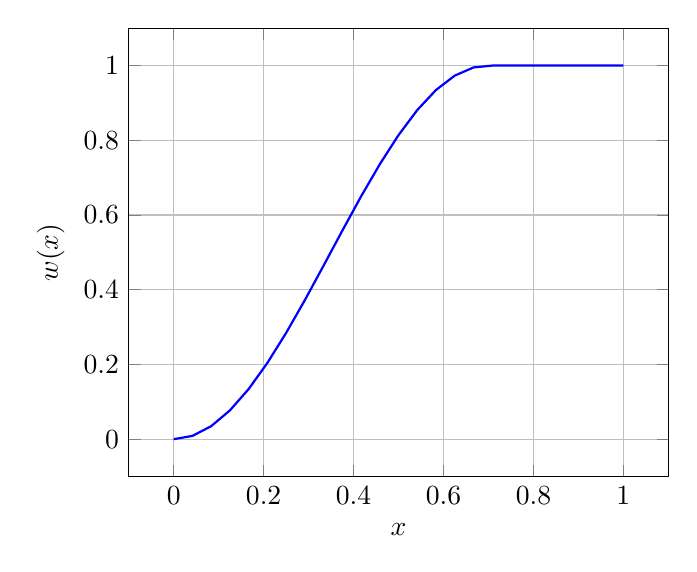
\begin{tikzpicture}[
		declare function={
			func(\x) = (\x >= 0.7) * (1) +
				and(\x < 0.7, \x >= 0) * (1/2 * sin(4.5 * deg(\x) - deg(pi)/2) + 1/2);
		}
	]
		\begin{axis}[
			xlabel=$x$, ylabel=$w(x)$,
			domain=0:1,
			grid = both,
			major grid style = {lightgray},
			minor grid style = {lightgray!25},
		]
			\addplot [blue,thick] {func(x)};
		\end{axis}
	\end{tikzpicture}
	\caption{Grafico della funzione di pesatura della I parte dell'\Cref{eq:weight-function}.}
	\label{graph:weight-function}
\end{figure}

Come si può osservare, applicare questa semplice funziona alla parte I dell'\Cref{eq:project-similarity} garantisce di attenuare il contributo dove il rapporto tra sorgenti riportati e sorgenti totali è esiguo ed enfatizzare i rapporti più elevati. 

% D'altro canto, l'obiettivo non è determinare tutte le similarità tra tutti i sorgenti, bensì avere un'indicazione dei progetti più simili e, perciò, presumibilmente copiati.

\section{Strumenti di sviluppo}

\subsection*{\textit{Kotlin}}
Il progetto è stato sviluppato interamente in \textit{Kotlin}, un linguaggio di programmazione \textbf{orientato agli oggetti} e \textbf{funzionale} \textit{open source}\footnote{\url{https://github.com/JetBrains/kotlin}} progettato e gestito da \textit{JetBrains}\footnote{\url{https://www.jetbrains.com/}} a partire dal 2010.
%
Si tratta di un linguaggio multipiattaforma compilato, tipato staticamente e  completamente interoperabile con \textit{Java} e la \textit{JVM} e \textit{Android}, applicabile in una vasta gamma di ambiti, dallo sviluppo \textit{server side} a quello di applicazioni mobili (attualmente è il linguaggio di riferimento per \textit{Android}, avendo surclassato Java).
%
Inoltre, oltre a Java e Android, \textit{Kotlin} può essere compilato in \textit{JavaScript}, consentendo di eseguire codice \textit{Kotlin} nel \textit{browser}.

L'obiettivo principale del linguaggio è fornire un'alternativa a Java più concisa, produttiva e sicura, adatta in tutti i contesti in cui è tutt'oggi utilizzato.
%
Infatti, essendo completamente compatibile con Java, sfrutta tutte le sue numerose librerie, estendendole e garantendo le stesse \textit{performance}.

I tratti distintivi di \textit{Kotlin} sono certamente la sua espressività e concisione, che permettono di sviluppare codice che rivela l'intento senza oscurarlo con codice verboso per specificare come viene realizzato.

\begin{figure}[h]
    \centering
    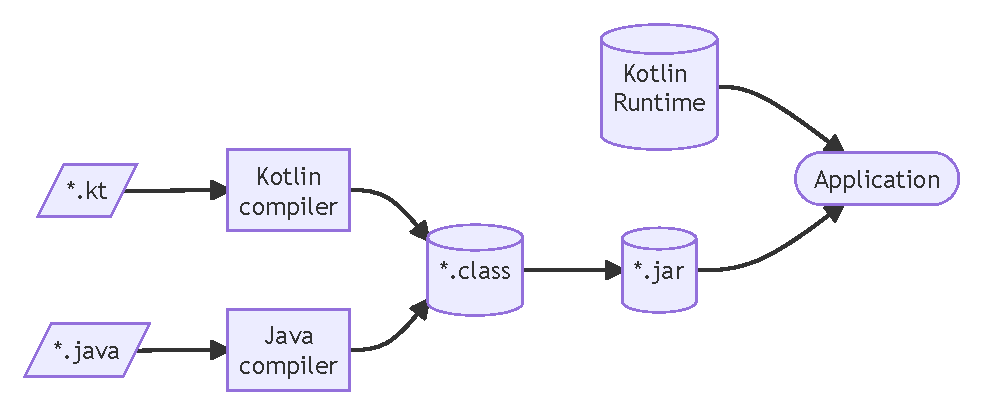
\includegraphics[width=0.8\textwidth]{resources/img/03-kotlincompilation.pdf}
    \caption{Processo di compilazione di \textit{Kotlin}.}
    \label{img:03-kotlin-compilation}
\end{figure}

\subsection*{Git e \textit{CI/CD}}
\label{03-git-ci}
Per lo sviluppo del progetto si è utilizzato Git, uno \textit{standard de facto} nell'ambito dei sistemi di controllo di versione decentralizzato, che permettere di tenere traccia dello storico delle modifiche e lo sviluppo simultaneo da parte di più sviluppatori, senza che questi debbano sobbarcarsi la gestione dell'intero progetto a mano, con tutti i conseguenti problemi.

In particolare, il \textit{workflow} adottato è il seguente: il progetto è mantenuto in una \textit{repository} pubblica centrale\footnote{\url{https://github.com/DanySK/code-plagiarism-detector}} e ciascun sviluppatore lavora su una \textit{working copy} (\textit{fork}).
%
Non appena una \textit{feature} è completata o si arriva a un buon grado di sviluppo si aprono delle \textit{pull request}, nelle quali i contributi sono revisionati per accertarsi passino i controlli di qualità.
%
Questi vengono eseguiti automaticamente grazie all'utilizzo delle \textit{GitHub Actions}, una piattaforma di \textit{Continuous Integration and Delivery} (\textit{CI/CD}) che permette di automattizare il processo di \textit{testing}, \textit{building} e \textit{deployment}.
%
Tramite un file di configurazione \textit{Yaml} è possibile definire uno o più \textit{workflow} che effettuino i controlli desiderati al verificarsi di alcuni eventi come, ad esempio, una \textit{pull request} o il \textit{push} di un nuovo commit.
%
In particolare, il progetto è configurato per eseguire i \textit{test} ad ogni \textit{commit} che viene \textit{pushato} su tutti e tre i sistemi operativi più diffusi, \textit{Linux}, \textit{MacOS}, \textit{Windows}, e per effettuare, ad ogni \textit{pull request}, ulteriori controlli come la copertura del codice in termini di test\footnote{\url{https://about.codecov.io/}} e la qualità del codice\footnote{\href{https://lift.sonatype.com/getting-started}{\texttt{Sonatype Lift}}} al fine di identificare problemi di sicurezza, prestazioni, affidabilità e stile.
%
Questo metodo di operare è alla base della filosofia \textit{DevOps} e prevede di verificare, ad ogni cambiamento, che la \textit{build} rimanga intatta, al fine di individuare eventuali problemi appena questi si verificano e non dopo settimane, al termine dell'integrazione.

\subsection*{Note di sviluppo}
\begin{itemize}
	\item La parallelizzazione dell'analisi dei sorgenti è stata sviluppata per mezzo di \textit{ParallelStream} il quale, a loro volta, fa uso di un \textit{framework} di tipo \textit{fork-join}, che ha l'onere di creare e dividere la computazione tra i vari \textit{thread} e gestire le relative \textit{join} in maniera trasparente allo sviluppatore. Per far ciò si è dovuto, tuttavia, prestare attenzione affinché gli algoritmi di \textit{detection} fossero \textit{thread-safe}.
	\item Per lo sviluppo complessivo del progetto sono state impiegate le seguenti librerie:
	\begin{itemize}
		\item \textbf{JavaParser}\footnote{\url{https://javaparser.org}} per effettuare l'analisi dei sorgenti sviluppati in linguaggio Java;
		\item \textbf{Github API for Java}\footnote{\url{https://github-api.kohsuke.org}} per interagire con l'API di GitHub e recuperare le \textit{repository}. Per recuperare i progetti caricati su \textit{Bitbucket}, non essendoci una libreria pronta all'uso, si è utilizzato \textbf{Unirest} per effettuare le richieste HTTP;
		\item \textbf{JGit}\footnote{\url{https://www.eclipse.org/jgit/}} per lo scaricamento (\textit{clone}) dei progetti da \textit{GitHub} e \textit{Bitbucket}.
		\item \textbf{Clikt}\footnote{\url{https://ajalt.github.io/clikt/}} per la scrittura dell'interfaccia da riga di comando;
		\item \textbf{Kaml}\footnote{\url{https://github.com/charleskorn/kaml}} per la (de)serializzazione di file di configurazione \textit{Yaml}.
		\item \textbf{Kotest}\footnote{\url{https://kotest.io}} e \textbf{Mockk}\footnote{\url{https://mockk.io}} per effettuare e agevolare la scrittura di \textit{test}.
	\end{itemize}
\end{itemize}

	% ! TeX root = ../../thesis.tex
\chapter{Validazione, conclusioni e lavori futuri}
\label{chapter:validation}
In questo capitolo vengono riportati e analizzati i risultati ottenuti nell'ambito di applicazione dello strumento sviluppato.

\section{Valutazione qualitativa}
Le prestazioni del sistema sono misurate sulla base di due aspetti fondamentali e indipendenti tra loro: le \textit{performance}, in termini di tempo d'esecuzione, ma soprattutto l'accuratezza.
%
Infatti, lo scopo primario è rilevare con precisione casi probabili di plagio e presentarli all'utente il più in alto possibile nei \textit{report} generati dallo strumento.
%
\`E solo in seguito ad aver raggiunto un grado di precisione soddisfacibile che possono essere adottate ottimizzazioni che permettano di ridurre il tempo di calcolo.

Dunque, per testarne l'accuratezza sono stati considerati 130 diversi progetti del corso di Programmazione ad Oggetti presentati nell'arco degli ultimi tre anni accademici e per ciascuno di questi si è effettuato il confronto con tutti i progetti a disposizione dal 2015 in poi che, complessivamente, ammontano a 354 progetti.
%
Questi sono sviluppati in Java, generalmente in \textit{team} di quattro componenti, e rappresentano artefatti di medio-alta complessità, costituiti in media da più di un centinaio di sorgenti ciascuno.

\subsection{Analisi di sensitività}
Dapprima si è testato il sistema eseguendo una scansione senza applicare alcun filtraggio intermedio delle rappresentazioni come descritto nella \Cref{03:filtering-phase}, scegliendo come parametri di riferimento i seguenti:
\begin{itemize}
    \item $s$, minima lunghezza della sequenza di \textit{token} rilevabile dall'algoritmo di \textit{detection} (\textit{RKR-GST}) pari a 15;
    \item valore di soglia percentuale sotto la quale la similarità di una coppia di sorgenti non viene segnalata pari al 30\%;
    \item metrica espressa dall'\Cref{eq:avg-norm-sim}.
\end{itemize}

A seguito dell'analisi si è effettuata un'ispezione manuale dei sorgenti in modo tale da verificare che le stime effettuate dallo strumento non fossero fuorvianti o prive di fondamento.

I risultati complessivi sono presentati in \Cref{table:results}; per semplicità sono riportati solo le corrispondenze con similarità maggiore del 40\%.

\begin{table}[h!]
    \centering
    \begin{tabular}{|p{0.2\linewidth}|p{0.2\linewidth}|p{0.15\linewidth}|p{0.35\textwidth}|}
        \hline
        \textbf{Progetto originale} & \textbf{Progetto copiato} & \textbf{Similarità} & \textbf{Ispezione manuale} \\ [0.5ex] 
        \hline\hline
        gym-man & gym-man & 100\% & corrispondenza totale \\
        \hline
        spacewar & Space-Invaders & 90\% & corrispondenza totale \\
        \hline
        zombiegame & boxhead & 81\% & corrispondenza elevata \\
        \hline
        paranoid & b.b.evo & 70\% & corrispondenza medio-alta \\
        \hline
        space-run & alone-in-the-space & 62\% & corrispondenza medio-alta \\
        \hline
        Flappy Bird & SMR & 55\% & corrispondenza parziale \\
        \hline
        Teatro & harbor-mgr & 49\% & corrispondenza parziale \\
        \hline
        ALA & traffic-sim & 48\% & nessuna corrispondenza - "falso positivo" \\
        \hline
    \end{tabular}
    \caption[Risultati ottenuti confrontando i progetti sottomessi negli ultimi tre anni accademici]{Risultati ottenuti confrontando i progetti consegnati negli ultimi tre anni accademici. Nell'ultima colonna vi è riportato l'esito dell'ispezione manuale eseguita a seguito di quella automatica; per semplicità si sono catalogate le corrispondenze in: corrispondenza \textit{totale}, \textit{elevata}, \textit{parziale} o \textit{falso positivo}.}
    \label{table:results}
\end{table}

Come si può osservare, lo strumento è in grado di rilevare molto bene copiature evidenti, ovvero casi in cui sono state copiate intere classi di sorgenti: è il caso dei primi due risultati in cui i progetti sono pressoché identici e la percentuale di similarità stimata non è inferiore al 90\%.
%
Nel secondo caso la similarità al 90\% è spiegabile dal fatto che alcune interfacce sono molto piccole e non hanno una lunghezza (in numero di \textit{token}) sufficiente per essere rilevate (cioè sono minori della minima lunghezza $s$ imposta nell'algoritmo \textit{Running Karp Rabin Greedy String Tiling}).

Come naturale che sia, invece, laddove la copiatura è effettuata in modo più scaltro, attingendo in modo parziale da altri progetti, la similarità cala, mantenendosi tuttavia al di sopra del 60\%.

Sotto il 60\% si è in presenza di codice piuttosto simile, ma in maniera molto limitata rispetto alla totalità dei sorgenti.
%
\`E il caso, ad esempio, dei progetti \texttt{SMR} e \texttt{Flappy Bird} in cui è intuibile, guardando i risultati generati dal rilevatore, che gli sviluppatori del secondo abbiano preso spunto dal primo.
%
Tuttavia non è ravvisabile una copiatura evidente come nei precedenti casi.

Un solo caso, tra tutti i progetti analizzati, riporta similarità maggiore del 45\% senza essere realmente copiato.
%
Ciononostante, la similarità riportata non è superiore al 50\% e il fatto che i progetti non siano copiati né simili è facilmente verificabile in pochi minuti guardando il \textit{report} stesso che comprende solo costanti e \textit{getter/setter}.

Successivamente, al fine di verificare la combinazione ottimale di parametri da utilizzare, sono state rieffettuate le scansioni dei soli progetti somiglianti presentati in \Cref{table:results}, facendoli opportunamente variare.
%
Come si può notare dalla \Cref{table:grid-search} le misurazioni di similarità più accurate in relazione all'ispezione manuale riportata in \Cref{table:results} sono in corrispondenza di una lunghezza\dots

Si noti che la misurazione della similarità mediante l'\Cref{eq:max-norm-sim} in concomitanza con quella dei progetti (\Cref{eq:project-similarity}) genera risultati fuorvianti in corrispondenza di piccoli progetti e/o sorgenti di piccola dimensione.
%
Questo fenomeno è facilmente osservabile dalle stime di similarità tra i progetti \texttt{Flappy-bird} e \texttt{SMR}. 
%
Questo ci spinge a preferire l'utilizzo della metrica descritta nell'\Cref{eq:max-norm-sim} piuttosto che...

\begin{landscape}
    \begin{table}[h!]
        \centering
        \begin{tabular}{ c|c|c|p{1cm}|p{1.5cm}|p{2cm}|p{1.5cm}|p{1.5cm}|p{1.5cm}|p{1.5cm}|p{1.2cm} }
            \multicolumn{3}{c|}{} & gym-man / gym-man & spacewar / space-invaders & zombiegame / boxhead & paranoid / b.b.evo & Space-run / alone-in-the-space & flappy-bird / SMR & Teatro / harbor-mgr & ALA / traffic-sim \\ [0.5ex]
            \hline\hline
            \multirow{6}{*}{$\text{min-dup}=0.3$} & \multirow{2}{*}{$s=15$} & Max & 100\% & 95\% & 72\% & 72\% & 75\% & 80\% & 56\% & 74\% \\
            & & Avg & 100\% & 90\% & 81\% & 70\% & 62\% & 55\% & 49\% & 48\% \\
            & \multirow{2}{*}{$s=20$} & Max & 100\% & 99\% & 72\% & 75\% & 63\% & 83\% & 50\% & 57\% \\
            & & Avg & 100\% & 91\% & 58\% & 71\% & 48\% & 61\% & 51\% & 31\% \\
            & \multirow{2}{*}{$s=25$} & Max & 100\% & 98\% & 54\% & 66\% & 49\% & 79\% & 46\% & 26\% \\
            & & Avg & 100\% & 92\% & 42\% & 58\% & 41\% & 51\% & 40\% & 12\% \\
            \hline

            \multirow{6}{*}{$\text{min-dup}=0.4$} & \multirow{2}{*}{$s=15$} & Max & 100\% & 96\% & 81\% & 76\% & 70\% & 79\% & 61\% & 75\% \\
            & & Avg & 100\% & 92\% & 73\% & 79\% & 57\% & 62\% & 55\% & 22\% \\
            & \multirow{2}{*}{$s=20$} & Max & 100\% & 99\% & 65\% & 85\% & 63\% & 80\% & 57\% & 47\% \\
            & & Avg & 100\% & 97\% & 49\% & 69\% & 44\% & 54\% & 39\% & 10\% \\
            & \multirow{2}{*}{$s=25$} & Max & 100\% & 99\% & 49\% & 64\% & 42\% & 80\% & 46\% & 64\% \\
            & & Avg & 100\% & 99\% & 36\% & 62\% & 34\% & 52\% & 20\% & 6\% \\
            \hline

            \multirow{6}{*}{$\text{min-dup}=0.5$} & \multirow{2}{*}{$s=15$} & Max & 100\% & 99\% & 80\% & 84\% & 64\% & 76\% & 67\% & 27\% \\
            & & Avg & 100\% & 99\% & 51\% & 73\% & 33\% & 52\% & 33\% & 14\% \\
            & \multirow{2}{*}{$s=20$} & Max & 100\% & 99\% & 56\% & 82\% & 59\% & 56\% & 45\% & 35\% \\
            & & Avg & 100\% & 99\% & 30\% & 67\% & 30\% & 47\% & 23\% & 4\% \\
            & \multirow{2}{*}{$s=25$} & Max & 100\% & 99\% & 44\% & 63\% & 38\% & 56\% & 27\% & 15\% \\
            & & Avg & 100\% & 98\% & 21\% & 55\% & 27\% & 47\% & 11\% & 3\% \\
            \hline
        \end{tabular}
        \caption[]{}
        \label{table:grid-search}
    \end{table}
\end{landscape}

Si è infine testato il risultato dell'analisi eseguendo il filtraggio delle rappresentazioni come descritto nella \Cref{03:filtering-phase}.

\begin{table}[h!]
    \centering
    \begin{tabular}{|c|c|c|c|c|}
        \hline
        \diagbox{\textbf{Progetti}}{\textbf{Soglia filtro}} & \textbf{assente} & \textbf{0,3} & \textbf{0,4} & \textbf{0,5} \\ [0.5ex] 
        \hline\hline
        gym-man - gym-man & 100\% & 100\% & 100\% & 100\% \\
        \hline
        spacewar - Space-Invaders & 90\% & 90\% & 90\% & 90\% \\
        \hline
        zombiegame - boxhead & 81\% & 81\% & 81\% & 80\% \\
        \hline
        paranoid - b.b.evo & 70\% & 70\% & 70\% & 78\% \\
        \hline
        space-run - alone-in-the-space & 62\% & 62\% & 62\% & 59\% \\
        \hline
        Flappy Bird - SMR & 55\% & 55\% & 55\% & 55\% \\
        \hline
        Teatro - harbor-mgr & 49\% & 49\% & 49\% & 49\% \\
        \hline
        ALA - traffic-sim & 48\% & 48\% & 48\% & 46\% \\
        \hline
    \end{tabular}
    \caption{}
    \label{table:filter-results}
\end{table}

\subsection{Analisi di sensibilità}

\section{Tempi d'esecuzione}
Per quanto concerne i tempi d'esecuzione, attualmente lo strumento impiega, per fare il confronto di un progetto con i 354 progetti disponibili, grazie alla parallelizzazione e al salvataggio in locale dei sorgenti da analizzare, mediamente un terzo del tempo che avrebbe impiegato senza effettuare il \textit{caching}, stimabile all'incirca in al più 20 minuti.
%
Questo dipende anche in maniera incontrollabile dal calcolatore su cui viene eseguito.

\section{Conclusioni}

\section{Sviluppi futuri}

	% --------------------------------------------------------------------
	% Backmatter command leaves the page numbering alone but switches the 
	% chapters back to being not numbered.
	% --------------------------------------------------------------------
	\nocite{*}
	{
		\backmatter	
		% % ! TeX root = ../../thesis.tex
\chapter{Conclusioni}
L'obiettivo della tesi, realizzare un sistema automatico per l'individuazione e il rilevamento di possibili plagi, è stato raggiunto.
%
La tecnica implementata, basata sull'analisi strutturale dei sorgenti, è in grado di rilevare evidenti copiature e parti molto simili, fornendo buoni risultati anche nei casi di copiature "intelligenti", laddove da parte degli sviluppatori c'è stata un'opera di rifattorizzazione mirata ad offuscare le copiature.

Le prestazioni, seppur non eccelse, garantiscono di eseguire lo strumento in tempi brevi

		% ----------------------------------------------------------------
		% Bibliography
		% ----------------------------------------------------------------
		\printbibliography
		% % ! TeX root = ../../thesis.tex
\chapter*{Ringraziamenti}
	}
	% --------------------------------------------------------------------
	% Appendix
	% --------------------------------------------------------------------
	\appendix
	% ! TeX root = ../../thesis.tex
\chapter{Esempio di \textit{report} generato dallo strumento}

Di seguito viene mostrato un esempio di porzione di \textit{report} generato dallo strumento sviluppato.

\lstinputlisting[]{resources/code/app-report-example.txt}
\end{document}
